\documentclass{article}
\usepackage{amsmath,amssymb,amsthm} % AMS styles for extra equation formatting
\usepackage{graphicx} % for including graphics files
\usepackage{subfig} % for subfigures
\usepackage[numbers,sort]{natbib} % for better references control
\usepackage{hyperref} % for hyperlinks within the paper and references
\usepackage{fontspec}  % Allows for system fonts
\usepackage[top=2cm, bottom=2cm, left=2cm, right=2cm]{geometry}  % Set margins on all sides
\usepackage{setspace} % for line spacing
\usepackage{appendix} % for the appendices
\usepackage{listings} % for code
\usepackage{xcolor} % for color
\usepackage{url,textcomp}
\usepackage{matlab-prettifier}
\usepackage{tabularx}
%%%%%%%%%%%%%%%%%%%%%%%%%%%%%%%%%%%%%%%%%%%%%%%%%%%%%%%%%%%%%%%%%%%%%%%%%%%%%%

\hypersetup{colorlinks=true, linkcolor=blue,  anchorcolor=blue,
citecolor=blue, filecolor=blue, menucolor=blue, pagecolor=blue,
urlcolor=blue}

%%%%%%%%%%%%%%%%%%%%%%%%%%%%%%%%%%%%%%%%%%%%%%%%%%%%%%%%%%%%%%%%%%%%%%%%%%%%%%

\newcommand{\todo}[1]{\vspace{5 mm}\par \noindent
\marginpar{\textsc{Todo}}
\framebox{\begin{minipage}[c]{0.90 \textwidth}
\tt \flushleft #1 \end{minipage}}\vspace{5 mm}\par}
\newcommand{\setParDis}{\setlength {\parskip} {0.2cm} } % for 0.3cm spacing
\newcommand{\setParDef}{\setlength {\parskip} {0pt} } % for 0 spacing

%%%%%%%%%%%%%%%%%%%%%%%%%%%%%%%%%%%%%%%%%%%%%%%%%%%%%%%%%%%%%%%%%%%%%%%%%%%%%%

\graphicspath{{graphics/}}

\newtheorem{theorem}{Theorem}[section]
\newtheorem{proposition}[theorem]{Proposition}
\newtheorem{lemma}[theorem]{Lemma}
\newtheorem{corollary}[theorem]{Corollary}
\newtheorem{definition}[theorem]{Definition}

%\renewcommand{\qedsymbol}{$\blacksquare$} % for filled square at end of proof
%\numberwithin{equation}{section} % for the 1.1, 1.2 equation number style
%\setlength{\parindent}{0em} % don't indent paragraphs
%\setlength{\parskip}{1em} % add spacing between paragraphs
%\linespread{1.6} % double-spacing

\setmainfont{Arial}
% \doublespacing
\onehalfspacing
\setcounter{secnumdepth}{3}

%%%%%%%%%%%%%%%%%%%%%%%%%%%%%%%%%%%%%%%%%%%%%%%%%%%%%%%%%%%%%%%%%%%%%%%%%%%%%%

\begin{document}

\title{%
Report for Speech Recognition \\
\large\itshape{EEEM030 - Speech Recognition - Group Assignment 2}}
\author{\normalsize\slshape{Group 1: Xiaoguang Liang, Tofarati Onatunde, Zeyad Adelmonem and Jaison Baptist Sequira}}
\date{\normalsize\slshape\today}
\maketitle


% Suppress any floats (figures, tables) from appearing on the next page
\suppressfloats

\tableofcontents

\begin{abstract}
Abstract
This report presents the implementation of a speech recognition system based on a Hidden Markov Model (HMM) for isolated word recognition. Utilizing precomputed Mel-Frequency Cepstral Coefficients (MFCCs) as features, the system incorporates feature normalization, parameter initialization for the HMM, sequence decoding via the Viterbi algorithm, and comprehensive evaluation metrics. The system’s performance is assessed through a recognition error rate and a confusion matrix, providing insights into its effectiveness in identifying words from a limited vocabulary. The implementation demonstrates the application of HMMs in speech recognition and highlights the impact of key steps such as initialization and decoding on system accuracy.

\end{abstract}

%%%%%%%%%%%%%%%%%%%%%%%%%%%%%%%%%%%%%%%%%%%%%%%%%%%%%%%%%%%%%%%%%%%%%%%%%%%%%%

\section{Introduction}
\setParDis

This assignment involves designing and implementing a basic speech recognition system using fundamental speech and audio processing techniques. The system, developed in MATLAB, performs isolated-word recognition for a vocabulary of eleven words, structured around five key tasks: feature extraction, model initialisation, training, evaluation, and testing. HMMs form the core methodology, providing a framework to explore the impact of maximum likelihood training on system performance. The recogniser uses the Baum-Welch algorithm and the Viterbi algorithm for decoding and recognising these words. The activities include within this coursework include:

\begin{itemize}
	\item \textbf{MFCC Feature Extraction:} for extracting acoustic features for training, evaluation, and additional test datasets.
	\item \textbf{HMM Initialisation and Training:} For initialising the prototype HMMs using global statistics of the training data. In addition to iteratively refining model parameters using forward-backward algorithms to compute likelihoods and re-estimate transitions and emissions.
	\item \textbf{Recognition and Evaluation:} for calculating the Viterbi likelihoods and decoding the recognition outputs. In turn scoring the system performance via confusion matrices and error rate calculations.
\end{itemize}


The contribution of members of our group is shown in Table \ref{table:report} and Table \ref{table:codes}.

\begin{table}[!h]
\caption{Contribution list of the written report} % title of Table
\centering % used for centering table
\label{table:report}
{
\begin{tabularx}{0.9\textwidth}[h]
 { 
  | >{\centering\arraybackslash}X 
  | >{\centering\arraybackslash}X | }
 \hline
 Section & Name \\
 \hline
 Abstract  & Tofarati Onatunde  \\
 \hline
 1 Introduction  & Tofarati Onatunde  \\
 \hline
 2  & Tofarati Onatunde  \\
 \hline
 3  & Xiaoguang Liang \\
 \hline
 4  & Zeyad Adelmonem  \\
 \hline
 5  & Jaison Baptist Sequira \\
 \hline
 6  & Xiaoguang Liang  \\
 \hline
 7 Conclusion  & Tofarati Onatunde  \\
 \hline
 \end{tabularx}
}
\end{table}


\begin{table}[!h]
\caption{Contribution list of codes} % title of Table
\centering % used for centering table
\label{table:codes}
{
\begin{tabularx}{0.9\textwidth}[h]
 { 
  | >{\centering\arraybackslash}X 
  | >{\centering\arraybackslash}X | }
 \hline
 Task & Name \\
 \hline
 1  & Tofarati Onatunde  \\
 \hline
 2  & Xiaoguang Liang  \\
 \hline
 3  & Zeyad Adelmonem \& Xiaoguang Liang \\
 \hline
 4  & Jaison Baptist Sequira \& Zeyad Adelmonem \& Xiaoguang Liang  \\
 \hline
 5  & Xiaoguang Liang \\
 \hline
 \end{tabularx}
}
\end{table}




%%%%%%%%%%%%%%%%%%%%%%%%%%%%%%%%%%%%%%%%%%%%%%%%%%%%%%%%%%%%%%%%%%%%%%%%%%%%%%

\section{Feature Extraction}

\subsection{Significance of Feature Extraction in Speech Recognition}
Feature extraction is an essential step in developing a speech recogniser system, as it transforms raw audio signals into a meaningful and compact interpretations that can be effectively processed by the speech recognition model.

Therefore, this section of the report will provide an overview of the underlying principles, processes and parameters used to extract 13 MFCCs including the zeroth coefficient, from the development and evaluation audio files sets, while supplementing relevant images of key results.

Before, explaining how the 13 MFCCs were extracted, it is vital to note that MFCC’s are widely regarded as the standard interpretation for speech recognition. This is because MFCC’s closely mimic the way the human ear process sound, by capturing the frequency spectrum of the audio signals on the Mel scale that closely aligns with the human auditory sensitivity to sound frequencies, while actively discarding irrelevant information such as pitch variations. Which works to retain essential phonetic features needed for distinguishing between speech sounds. 

\subsection{Audio Data Setup}


\begin{figure}[!tbp]
  \centering
  \subfloat[sp15a\_w02\_heed.mp3]{\includegraphics[width=0.32\textwidth]{audio1}\label{fig:female-segment-50ms}}
  \hfill
  \subfloat[sp01a\_w02\_hod.mp3]{\includegraphics[width=0.32\textwidth]{audio2}\label{fig:female-segment-200ms}}
  \hfill
  \subfloat[sp30a\_w02\_heard.mp3]{\includegraphics[width=0.32\textwidth]{audio3}\label{fig:female-order-15}}
  \hfill
  \caption{\label{fig:audio} Audio Signals of sound samples from the Developmet data set.}
\end{figure}

As shown in Appendix B Code \ref{lst:shared_feature_extraction}, the MATLAB code begins by defining 30 speakers used in the development data set and listing their repeated eleven-word vocabulary collections: "heed, hid, head, had, hard, hud, hod, hoard, hood, whod, and heard". Resulting in the 330 audio files showcasing variations in vowel sounds, constants and language articulations, ideal for studying phonetic features, visually represented by figure \ref{fig:audio}.

\paragraph{Note:} As shown in Appendix B, two \verb+for+ loops were used which generated filenames for all speaker-word combinations. Resulting in paths to all audio files, ensuring an organised dataset for subsequent processing. Each file followed the naming convention \verb+spXXa_wYY_word.mp3+, where: "XX" is the speaker index, "YY" is the word index, and "word" is the spoken terminology.

\subsection{MFCC Extraction Process}

Therefore, to initialise the feature extraction of the 13 MFCCs, including the zeroth coefficient, from the development set, and later the evaluation set, a few steps had to be taken, and are described below. 

\subsubsection{Frame and Hop Size Parameters}

The process begins with segmenting the audio signals into overlapping frames, each 30ms in duration. This temporal resolution corresponds to the typical length of phonemes, ensuring that each frame captures meaningful variations in speech without losing important details. Additionally, a hop size of 10ms with a 20ms overlap between consecutive frames was implemented. As this provided smooth transitions and comprehensive temporal coverage between frames. Overlapping frames are crucial in speech processing as they capture the continuity of spoken words, avoiding information loss between frames.

\subsubsection{Hamming Window for Spectral Analysis}

\paragraph{Note:} A Hamming window was also applied to each frame to reduce spectral leakage caused by transitions and abrupt frame boundaries. This step was utilised to improve the accuracy of frequency domain analysis, ensuring that the extracted features are reliable and precise.

\subsubsection{MFCC Calculation}

Finally, a built-in MATLAB function was implemented to extract the final MFCC values from each frame. Providing a compact yet detailed representation of the speech signal that focusing on the spectral content most relevant to human perception. It utilised the previously specified frame size, hop size, and the Hamming window to ensure high-quality feature extraction. The resulting 13-dimensional feature vector for each frame captures the static spectral characteristics of the speech signal. Then process was repeated for the evaluation set of audio samples.

Take note that delta and delta-delta features (velocities and accelerations) were excluded from the overall calculation of the MFCC’s. This simplification allows the code to focus on the static spectral characteristics of the audio signals. Which in turn improves computational efficiency while also maintaining sufficient information for effective speech recognition.

\subsection{Visualisation of Results}

After extracting the MFCC features for development and evaluation audio sets, several visualisations were created to illustrate the properties of the extracted features. Note: These graphs shown in this subsection were produced for all audio samples. However, only images pertaining to audio \verb+sp01a_w01_heed.mp3+ will be shown for simplification purposes.

\subsubsection{Audio Waveform to MFCC Spectrogram}

\begin{figure}[!h]
\begin{center}
\includegraphics[width=0.8\textwidth]{waveform}
\end{center}
\caption{\label{fig:waveform} Audio Waveform of sp01a\_w01\_heed.mp3.}
\end{figure}

By sourcing the length of the audio signal and plotting it against its linear amplitude,  a graph (Figure \ref{fig:waveform}) providing a time-domain representation of the heed speech signal showcasing its temporal variations and intensity was made.

\begin{figure}[!h]
\begin{center}
\includegraphics[width=0.8\textwidth]{mfcc}
\end{center}
\caption{\label{fig:mfcc} MFCC spectrogram of sp01a\_w01\_heed.mp3.}
\end{figure}

After putting the original audio signal, through the MFCC process described in \textit{Section 1.3}, the corresponding MFCCs can be displayed in a spectrogram-like image (Figure \ref{fig:mfcc}). Where the x-axis represents the frame index (time), and the y-axis illustrates the MFCC coefficients and the colour intensity indicates the magnitude. This visualisation provides a view of how the audios spectral content evolves over time.


\subsubsection{Spectrogram of the Audio Signal}

\begin{figure}[!h]
\begin{center}
\includegraphics[width=0.8\textwidth]{spectrogram}
\end{center}
\caption{\label{fig:spectrogram} MFCC spectrogram of sp01a\_w01\_heed.mp3.}
\end{figure}

Additionally, another spectrogram (Figure \ref{fig:spectrogram}) can be made to visualises the frequency domain of the signal over time. In turn, offering insights into the full frequency spectrum of the audio data.


\subsubsection{Evolution of MFCC Coefficients}

\begin{figure}[!h]
\begin{center}
\includegraphics[width=0.8\textwidth]{coefficient}
\end{center}
\caption{\label{fig:coefficient} Evolution of the first MFCC coefficent.}
\end{figure}

Moreover, the evolution (Figure \ref{fig:coefficient}) of the first MFCC coefficient can be plotted over time to highlight its dynamic behaviour across frames. This helps to emphasis the temporal variations in spectral content, which can be utilised when distinguishing between different speech sounds.


\subsubsection{Histogram of MFCC Coefficients}

\begin{figure}[!h]
\begin{center}
\includegraphics[width=0.8\textwidth]{histogram}
\end{center}
\caption{\label{fig:histogram} Histogram of sp01a\_w01\_heed.mp3 MFCC coefficents.}
\end{figure}

The histogram (Figure \ref{fig:histogram}) of the first MFCC coefficient shows its distribution across frames. This statistical representation reveals the range and frequency of phonetic feature values, thus providing insight into the acoustic properties of each speech signal.


\subsubsection{3D Plot of MFCC Features}

\begin{figure}[!h]
\begin{center}
\includegraphics[width=0.8\textwidth]{3D}
\end{center}
\caption{\label{fig:3D} 3D Plot of sp01a\_w01\_heed.mp3 MFCC Features.}
\end{figure}

Lastly, a 3D mesh plot (Figure \ref{fig:3D}) can be used to visualise the first three MFCC coefficients across time. Thus, illustrating the relationships between coefficients and their temporal evolution, offering a more comprehensive view of the feature space.

These images are useful in analysing and refining the extracted features, because: 
\begin{itemize}
	\item (a) The MFCC spectrogram highlights phonetic variations.
	\item (b) The waveform and audio spectrogram offer complementary views of the signal’s temporal and frequency characteristics.
	\item (c) The coefficient evolution and histograms reveal trends and statistical properties, aiding in fine-tuning recognition models.
\end{itemize}


In turn allowing us to understand MFCC features and how they evolve over time. They provide valuable insights for further model development, enabling applications such as automatic speech recognition (ASR), speaker identification, and audio classification.

To conclude this section, feature extraction detailed lays the foundation for an effective speech recognition system. Demonstrating the power of how extracting the MFFC’s creates a well-suited starting point for capturing meaningful information from speech signals and training HMMs, of which are detailed in later sections of this report. 






\section{Model initialization}


\subsection{Paremeters of HMM initialization}

Model initialization represents a fundamental stage in the training of HMMs. The efficacy of training algorithms such as the Baum-Welch algorithm is contingent upon the initialisation of model parameters in an optimal manner. These parameters encompass the initial state probabilities, represented by the symbol $\pi$, the state transition probabilities $A$, and the observation probabilities $B$. The implementation of an appropriate initialisation strategy provides a robust foundation for optimisation, whilst simultaneously preventing the convergence to suboptimal solutions. 

\paragraph{Initial State Probabilities $\Pi$:}
	 $\Pi = [\pi_1, \pi_2, \dots, \pi_N]$ represents the probability of starting in each state $i$ , where  $N$ is the number of states.
As indicated in the assignment document, the initial value of $\Pi$ is provided as follows:
\begin{equation}
\label{eqn:pi}
\pi_i = \begin{bmatrix}
 	1 & 0 & 0 & 0 & 0 & 0 & 0 & 0
 \end{bmatrix}
\end{equation}

\paragraph{State Transition Probabilities $A$:}
 $A = [a_{ij}]$  represents the probability of transitioning from state $i$ to state $j$, satisfying $\sum_{j=1}^N a_{ij} = 1$  for all $i$.
Here, initial $A$ is provided in the assigment document:
\begin{equation}
\label{eqn:A}
a_{ij} = \begin{bmatrix}
 	0.8 & 0.2 & 0 & 0 & 0 & 0 & 0 & 0 \\
 	0 & 0.8 & 0.2 & 0 & 0 & 0 & 0 & 0 \\
 	0 & 0 & 0.8 & 0.2 & 0 & 0 & 0 & 0 \\
 	0 & 0 & 0 & 0.8 & 0.2 & 0 & 0 & 0 \\
 	0 & 0 & 0 & 0 & 0.8 & 0.2 & 0 & 0 \\
 	0 & 0 & 0 & 0 & 0 & 0.8 & 0.2 & 0 \\
 	0 & 0 & 0 & 0 & 0 & 0 & 0.8 & 0.2 \\
 	0 & 0 & 0 & 0 & 0 & 0 & 0 & 0.8
 \end{bmatrix}
\end{equation}

\paragraph{Observation Probabilities $B$:}
 $B$ represents the probability of observing data given a state. For continuous observations, this is computed using a multivariate Gaussian probability density function $PDF$.
 
 The observation probability for a given state $i$ and observation $x$ is defined as \citep{EEEM030}:
\begin{equation}
B_i(x) = \frac{1}{(2\pi)^{d/2} |\Sigma_i|^{1/2}} e^{-\frac{1}{2}(x - \mu_i)^T \Sigma_i^{-1} (x - \mu_i)}
\end{equation}

where:
\begin{itemize}
\item $\mu_i$ is the mean vector for state $i$,
\item $\Sigma_i$ is the covariance matrix for state $i$,
\item $d$ is the dimensionality of the observation vector.
\end{itemize}

In practice:
\begin{itemize}
\item $\mu_i$ can be initialized as the global mean of the observations.
\item $\Sigma_i$ can be initialized as a diagonal matrix where diagonal entries are the variances of the clustered observations.
\end{itemize}

\subsection{Initializaton for Multivariate Gaussian PDF}

In models with multivariate Gaussian probability density functions (PDFs), the initialisation of model parameters is of critical importance for the success of the training process, particularly when using iterative algorithms such as the Baum-Welch algorithm. The process of initialization provides the model with initial estimates for the emission probabilities, which are represented as Gaussian distributions, as well as the transition probabilities and initial state probabilities \citep{HTK}.

The initialisation of the multivariate Gaussian PDF necessitates the estimation of the mean vector, designated as $\mu$, and the covariance matrix, designated as $\Sigma$, for each state within the HMM. These parameters serve to characterise the probability distribution of the observed data within each state \citep{EEEM030}.

\subsubsection{Segments splitting for data}
Divide the length of the feature data evenly into $N$ parts, where $N = 8$, representing the number of hidden states. This converts the training samples into an $8N\times13$matrix, facilitating the computation of the Multivariate Gaussian PDF.

\subsubsection{Calculation for mean}
To meet the requirements of this assignment, the feature data must be divided into $N$ segments to calculate a $13\times13$ mean matrix. Each segment is processed iteratively to compute the mean. For a matrix $X$ of size $m \times n$, the mean of each row is:
\begin{equation}	
\mu_i = \frac{1}{n} \sum_{j=1}^{n} X_{i,j}, \quad i = 1, 2, \ldots, m
\end{equation}

\subsubsection{Calculation for variance}
To meet the requirements of this assignment, the diagonal of the $13\times13$ covariance matrix is computed by splitting the feature data into $N$ segments, following the same approach as used for calculating the mean. Each segment is processed iteratively to compute the covariance matrix. For a matrix $X$ of size $m \times n$, the variance of each row is:
\begin{equation}	
Varrow(X) = \frac{1}{n} \sum{j=1}^n \left(X_{ij} - \mu_i\right)^2, \quad i = 1, 2, \dots, m
\end{equation}
where $\mu_i$ is the mean of the $i$-$th$ row.

\subsection{Normalization and regularization}
\paragraph{Normalization:} Normalize the input data to have zero mean and unit variance to ensure robust parameter estimation. In practice, Min-Max Normalization is implemented. Scales all elements to the range [0, 1] like this:
\begin{equation}
\text{Normalized Value} = \frac{\text{Value} - \text{Min}}{\text{Max} - \text{Min}}
\end{equation}

\paragraph{Regularization:} Regularizing the covariance matrix can prevent issues like singular matrices or overfitting. A small value epsilon is added to the diagonal elements of the covariance matrix:
\begin{equation}
\text{Regularized Matrix} = \text{Covariance Matrix} + \epsilon \cdot I
\end{equation}
where $I$ is the identity matrix.







\section{Model training with HMMs}

The Baum-Welch approach, which effectively estimates model parameters through an iterative Expectation-Maximization process, is the mainstay of HMM training. In order to prevent numerical underflow, we used a scaling factor. The algorithm uses both the Forward and Backward procedures to compute intermediate variables. These calculations make it possible to calculate two essential elements that are essential for parameter re-estimation: occupation likelihoods (state probabilities) and transition likelihoods (state transition probabilities). Using the determined likelihoods to optimize the likelihood of witnessing the training sequences, the procedure iteratively finetunes the parameters (transition and emission probabilities) until convergence as shown in Figure \ref{fig:HMM}.

\begin{figure}[!ht]
\begin{center}
\includegraphics[width=\textwidth]{HMM}
\end{center}
\caption{\label{fig:HMM} HMM training algorithm.}
\end{figure}


\subsection{Forward algorithm}

By employing dynamic programming, the Forward algorithm effectively determines the 
probability of an observation sequence in a Hidden Markov Model without resorting to the 
exponential difficulty of adding up every potential state sequence. It functions in three 
essential steps:

\paragraph{Initialization Step:} The procedure calculates the initial probability for each state 𝑖 for the first observation by multiplying two terms: the likelihood that state I would emit the first observation $b_i(o_1)$ and the probability of starting in state $i(\pi_i)$ \citep{jm3}.

\begin{equation}
\label{equ:initial-prob}
\alpha^r_1(i) = \pi_ib_i(o^r_i)
\end{equation}

\paragraph{Recursion Step:} The algorithm considers every path that could lead to each current state for each succeeding time step. It calculates the probability for each state $j$ at time $t$ by taking into account Previous state probabilities $\alpha_{t-1}(i)$. Transition probabilities $a_{ij}$ and Emission probability of current observation $b_j(o^r_t)$.

\begin{equation}
\label{equ:initial-prob}
\alpha^r_1(j) = \left[\sum^N_{i=1}\alpha^r_{t-1}a_{ij}\right]b_i(o^r_i), \quad t = 1, 2, \ldots, T
\end{equation}

\paragraph{Termination Step:} The terminal forward variables for each of the possible end states are added up to determine the final probability of the complete observation sequence.

\begin{equation}
	P^r = P(\mathcal{O}|\lambda) = \sum^N_{i=1}\alpha^r_T(i)\eta_i
\end{equation}

Without explicitly listing every conceivable state sequence, this method effectively builds on previously determined values to compute the overall likelihood by accumulating probabilities throughout the process.


\subsection{Backward algorithm}

Similar to its Forward counterpart, the Backward method uses dynamic programming to calculate the likelihood of a sequence in a Hidden Markov Model, but it operates in the opposite way. It functions as follows:

\paragraph{Initialization Step:} The procedure initializes the backward variables for every state with a value of $\eta$ at the last observation time $T$. Our starting point for moving backward through the sequence is established by this initialization.

\begin{equation}
	\beta^r_T(i) = \eta_i
\end{equation}


\paragraph{Recursion Step:} The Backward algorithm's recursive computation from the final time step backwards is the fundamental component of its dynamic programming methodology. By taking into account all potential future routes, the algorithm determines the probability of producing the remaining observations for each state at each time step prior to $T$. We take into consideration the probability of transitioning to any possible next state, the probability that the next state would emit the next observation we actually see, and the probability of generating all remaining observations from that next state in order to account for all possible paths leading from each current state. By going backwards through the observation series, this recursive approach effectively combines probability without explicitly listing every possibility, accumulating information about likely state sequences.

\begin{equation}
\beta^r_1(i) = \sum^N_{j=1}a_{ij}b_j(o^r_{t+1})\beta^r_{t+1}(j), \quad t = T-1, T-2, \ldots, 1
\end{equation}


\paragraph{Termination Step:} The Backward algorithm's Termination step calculates the overall probability of the observation sequence by considering the initial state probabilities. After computing all backward variables back to time $t=1$, we can obtain the total probability of our observation sequence by combining the initial state probabilities, the emission probabilities of the first observation, and the backward variables at time $t=1$ for all possible states. This combination gives us the same total probability as the Forward algorithm, just computed in the reverse direction.


\begin{equation}
	P^r = \sum^N_{i=1}\pi_ib_i(o^r_1)\beta^r_1(i)
\end{equation}


\subsection{Underflow problem}

Both forward and backward algorithms in HMM encounter underflow issues when they constantly multiply probabilities, producing incredibly small quantities that are impossible for computers to process correctly. We employ scaling factors at each time step t to solve this. To maintain the values within a calculable range, we multiply the forward variables $\alpha^r_t(i)$ and backward variables $\beta^r_t(i)$ by a scaling coefficient $c_t$. To ensure consistency, the same scaling factors are applied to both algorithms, and these scaling coefficients are utilized to determine the final probability \citep{1162264}.

Forward scaling:

\begin{equation}
	c_t = \frac{1}{\sum^N_{i=1}\alpha(i)}
\end{equation}

\begin{equation}
	\alpha(i) = c_t * \alpha(i)
\end{equation}

Backward scaling:

\begin{equation}
	\beta_t(i) = c_t * \beta(i)
\end{equation}

\subsection{Occupation likelihoods}

complete observation sequence, is estimated in HMM after forward and backward variables have been calculated. It integrates data from backward variables $\beta_t(i)$, which takes future observations into account, and forward variables $\alpha(i)$, which takes observations up to time $t$ into account. Each state's forward and backward variables are multiplied, and the result is normalized by the observation sequence's overall probability. Considering every observation, this gives a comprehensive picture of state occupancy. Understanding the most likely state sequence that produced the observations and re-estimating parameters in the Baum-Welch algorithm depend on these occupation probabilities.

\begin{equation}
	\gamma_t(i) = \frac{\alpha_t(i)\beta(i)}{P(\mathcal{O}|\lambda)}
\end{equation}


\subsection{Transition likelihoods}

Given the complete observation sequence and model parameters, transition likelihood estimation determines the probability of being in state $i$ at time $t$ and changing to state $j$ at time $t+1$. Forward variables $\alpha_{ij}$, backward variables $\beta_j(o_{t+1})$, transition probabilities $a_{ij}$and emission probabilities $\beta_j(o_{t+1})$ are used to calculate this probability. Utilizing forward variables, the computation takes into account the likelihood of staying in state $i$ until time $t$, transitioning to state $j$, producing the observation at $t+1$, and then utilizing backward variables to account for all further observations from $t+1$ onward. During the parameter re-estimation stage of the Baum-Welch method, these transition likelihoods are essential for updating the transition probability matrix.

\begin{equation}
	\xi_t(i,j) = \frac{\alpha_{t-1}(i)a_{ij}b_j(o_t)\beta_t(j)}{P}
\end{equation}

\subsection{Re-estimation}

Using the occupation and transition likelihoods that were previously determined, the re-estimation stage of the HMM (Baum-Welch algorithm) modifies the model parameters $\lambda = \{A, B, \pi\}$. The occupation likelihood at $t = 1$ is used to update the initial state probabilities $\pi$. To re-estimate the transition probabilities 𝐴, $\xi_t(i,j)$ and $\gamma_t(i)$ are used to calculate the ratio of expected transitions between states to total transitions from the source state. By using $\gamma_t(i)$ to compare observation occurrences in each state to total state occupations, the emission probabilities $B$ are updated. The new model $\gamma'$ formed by these modified parameters raises the likelihood $P(\mathcal{O}$ till convergence.






\section{Evaluation}

\subsection{Viterbi Algorithm}
The Viterbi algorithm is used for decoding the sequence of hidden states given the observation sequence. The algorithm uses dynamic programming to compute the maximum likelihood of the entire sequence by recursively calculating the most probable state at each time step.

\paragraph{Steps of the Viterbi Algorithm:}
\begin{enumerate}
\item \textbf{Initialization:} At time t=1, the probability of each state is computed using the initial state probabilities $\Pi$ and the emission probabilities $B$.
\item \textbf{Recursion:} For each subsequent time step t, the algorithm computes the maximum probability of each state by considering all transitions from previous states. This is done by combining the previous state’s probability and the transition probability.
\item \textbf{Termination:} After processing all time frames, the algorithm selects the state with the highest probability at the final time frame.
\item \textbf{Backtracking:} The state sequence is traced back using the back pointer matrix, which keeps track of the state transitions that led to the optimal path.
\end{enumerate}

\paragraph{Numerical Stability:}
To avoid underflow issues, probabilities are represented in logarithmic space. This ensures that the product of small probabilities does not result in numerical errors. Instead of multiplying probabilities, we add their logarithms.

By monitoring the optimal route to every state at every time step, the Viterbi algorithm determines the most likely state sequence in HMM. It employs a dynamic programming technique with two primary variables: $\psi_t(i)$ holds the prior state that resulted in this highest probability, and $\delta_t(i)$ indicates the highest likelihood of a path terminating in state $i$ at time $t$. As it advances through time, the algorithm uses emission probabilities $b_j(o_t)$ and transition probabilities $a_{ij}$ to calculate these variables. It requires scaling in order to avoid underflow, just like forward-backward algorithms. It finds the ideal state sequence by going back through $\psi_t(i)$ after arriving at the last observation. We have used logarithmic transformation and sum of logs instead of scaling as in forward and backward algorithms \citep{HMM}.






\subsection{Evaluation on the development set}

Upon analyzing the data, the development set consists of 30 groups, each containing 11 samples representing the pronunciations of 11 words spoken by the same individual. The dataset includes three voice types: male, female, and children. Specifically, there are 14 groups of male voices, 15 groups of female voices, and 1 group of children’s voices. To ensure a balanced distribution of training and testing data across different voice types, the development set is split based on gender. Since there is only one group of children’s voices, it is included in the training set. The training set comprises 80\% of the development set.

\paragraph{Recognition error rate:} This is the percentage of misclassified predictions in the test set compared to the ground truth. The formula for calculating the error rate is:
\begin{equation}
	Error Rate = \frac{Number of Incorrect Predictions}{Total Predictions}
\end{equation}

\paragraph{Confusion Matrix:} A confusion matrix is a table used to describe the performance of a classification model. Each row represents the true labels, while each column represents the predicted labels. It helps visualize the types of misclassifications made by the model.

In accordance with the specifications set forth in the assignment, the HMM model was trained for a total of 15 epochs. The error rates are calculated on the basis of the outputs of the Viterbi algorithm, and the resulting error rates on the development set are presented in the accompanying Figure \ref{fig:error-rate} and the error rates data is in the Table \ref{table:error-rates}.

From Figure \ref{fig:error-rate}, it can be seen that the error rates fluctuate around 0.4 as the epochs increase, reaching the lowest value of 0.363636 at the 11th epoch. This indicates that the model’s performance does not necessarily improve with an increasing number of epochs. The reasons for this include the following:

\begin{itemize}
	\item \textbf{Overfitting:} As the training progresses, the model may start overfitting the training data, capturing noise or irrelevant patterns instead of generalizable features. This reduces its ability to perform well on unseen data.
	\item \textbf{Local Minima or Suboptimal Convergence:} The optimization process (e.g., Baum-Welch algorithm) may converge to a local minimum or suboptimal solution. This could prevent the model from finding the best parameter settings, even with more epochs.
	\item \textbf{Lack of Sufficient Data Augmentation:} If the dataset is not sufficiently diverse or augmented, the model may not learn robust features. Consequently, additional training epochs will not improve performance significantly.
	\item \textbf{Learning Rate and Parameter Initialization:} Poorly chosen learning rates or suboptimal initial parameter values (e.g., transition probabilities, emission probabilities) can lead to slow or ineffective learning during training.
	\item \textbf{Plateauing of Performance:} HMMs may reach a plateau in performance, where further training does not lead to significant improvement because the model has already captured all the learnable patterns in the data.
\end{itemize}

\begin{figure}[!h]
\begin{center}
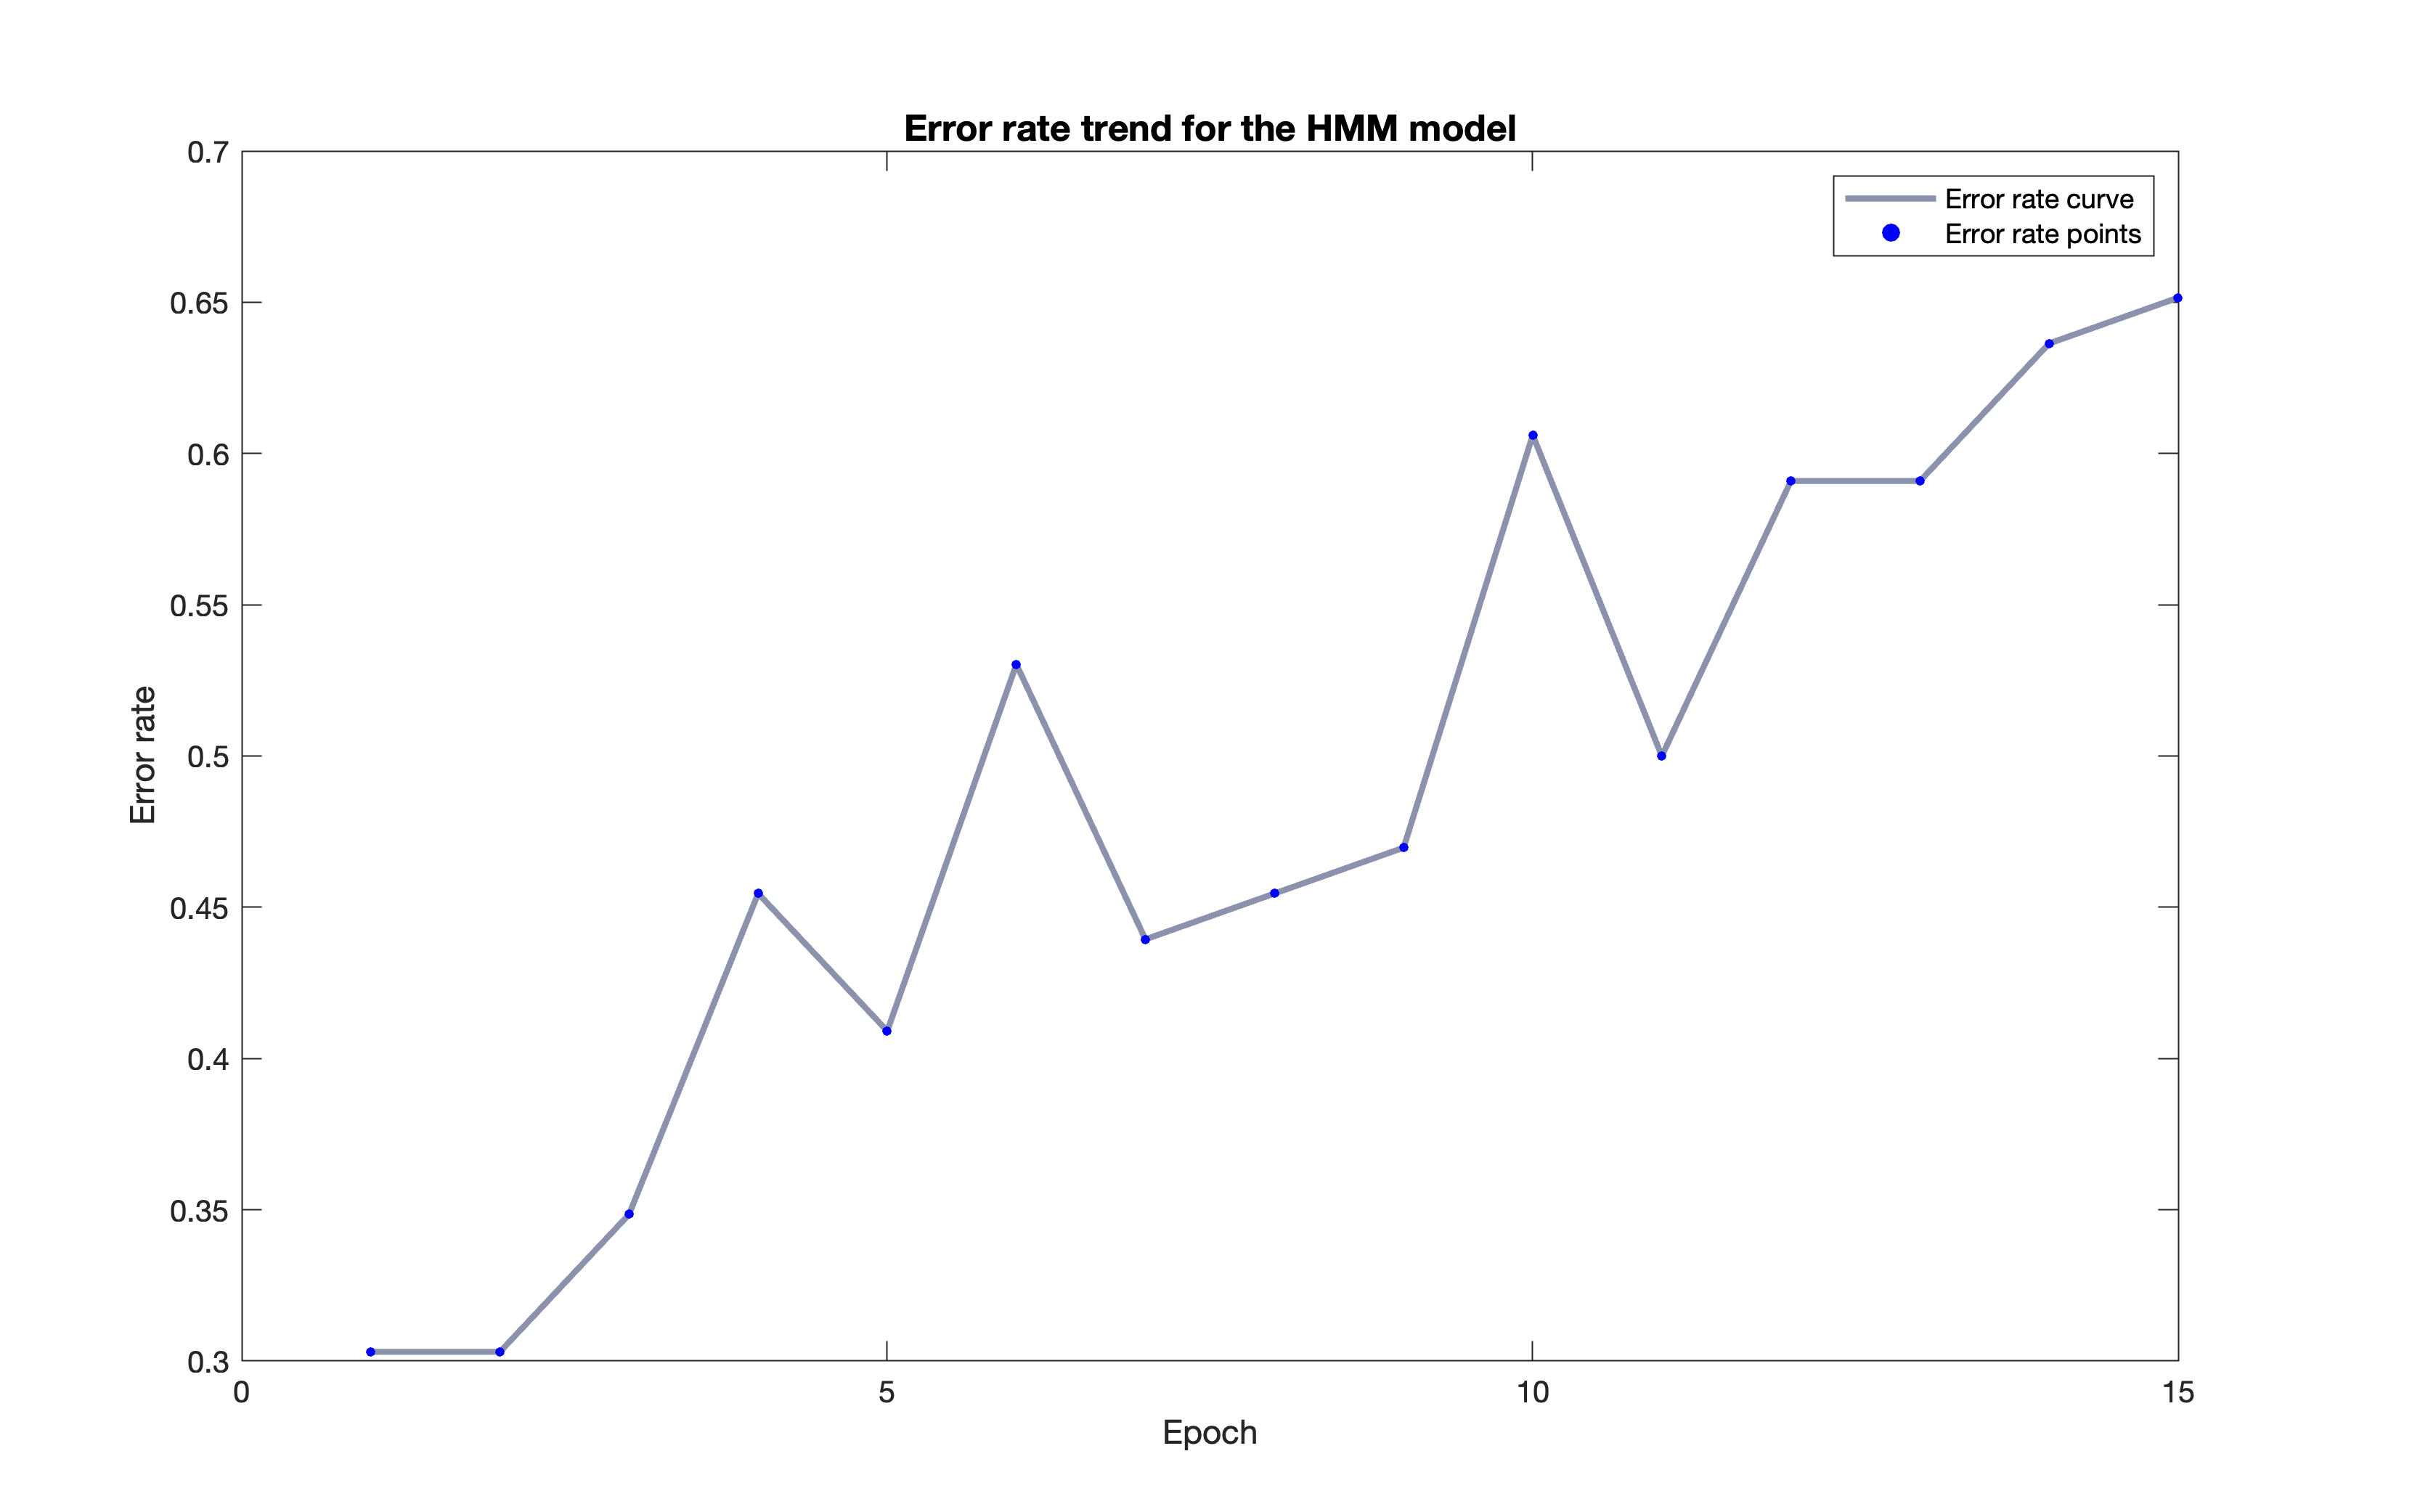
\includegraphics[width=\textwidth]{Error_rate_trend_for_HMM_model}
\end{center}
\caption{\label{fig:error-rate} Error rate trend for HMM model training on the development set.}
\end{figure}


\begin{table}[h]
\caption{Error rates for HMM model training on the development set} % title of Table
\centering % used for centering table
\label{table:error-rates}
{
\begin{tabularx}{0.5\textwidth}[h]
 { 
  | >{\centering\arraybackslash}X 
  | >{\centering\arraybackslash}X | }
 \hline
 Epoch & Error rate\\
 \hline
 1  & 0.393939  \\
 \hline
 2  & 0.393939  \\
 \hline
 3  & 0.5 \\
 \hline
 4  & 0.530303  \\
 \hline
 5  & 0.424242  \\
 \hline
 6  & 0.5  \\
 \hline
 7  & 0.409091  \\
 \hline
 8  & 0.454545  \\
 \hline
 9  & 0.393939 \\
 \hline
 10  & 0.424242  \\
 \hline
 11  & 0.363636  \\
 \hline
 12  & 0.424242  \\
 \hline
 13  & 0.424242 \\
 \hline
 14  & 0.515152  \\
 \hline
 15  & 0.424242  \\
 \hline
\end{tabularx}
}
\end{table}



\subsection{Evaluation on the evaluation set}

The evaluation is conducted on the evaluation set provided in the assignment. To ascertain the accuracy of the HMM model, the maximum cumulative likelihoods are initially calculated using the Viterbi algorithm. Subsequently, the accuracy is calculated based on the output of the Viterbi algorithm. The most optimal HMM model exhibits an accuracy of 0.318182 on the evaluation set. The equation for calculating accuracy is as follows:

\begin{equation}
	Accuracy = \frac{Number of Correct Predictions}{Total Predictions}
\end{equation}

The recognition outputs should be evaluated and a confusion matrix generated. The corresponding confusion matrix is presented in graphical form in Figure \ref{fig:confusion-matrix}.

\begin{figure}[!h]
\begin{center}
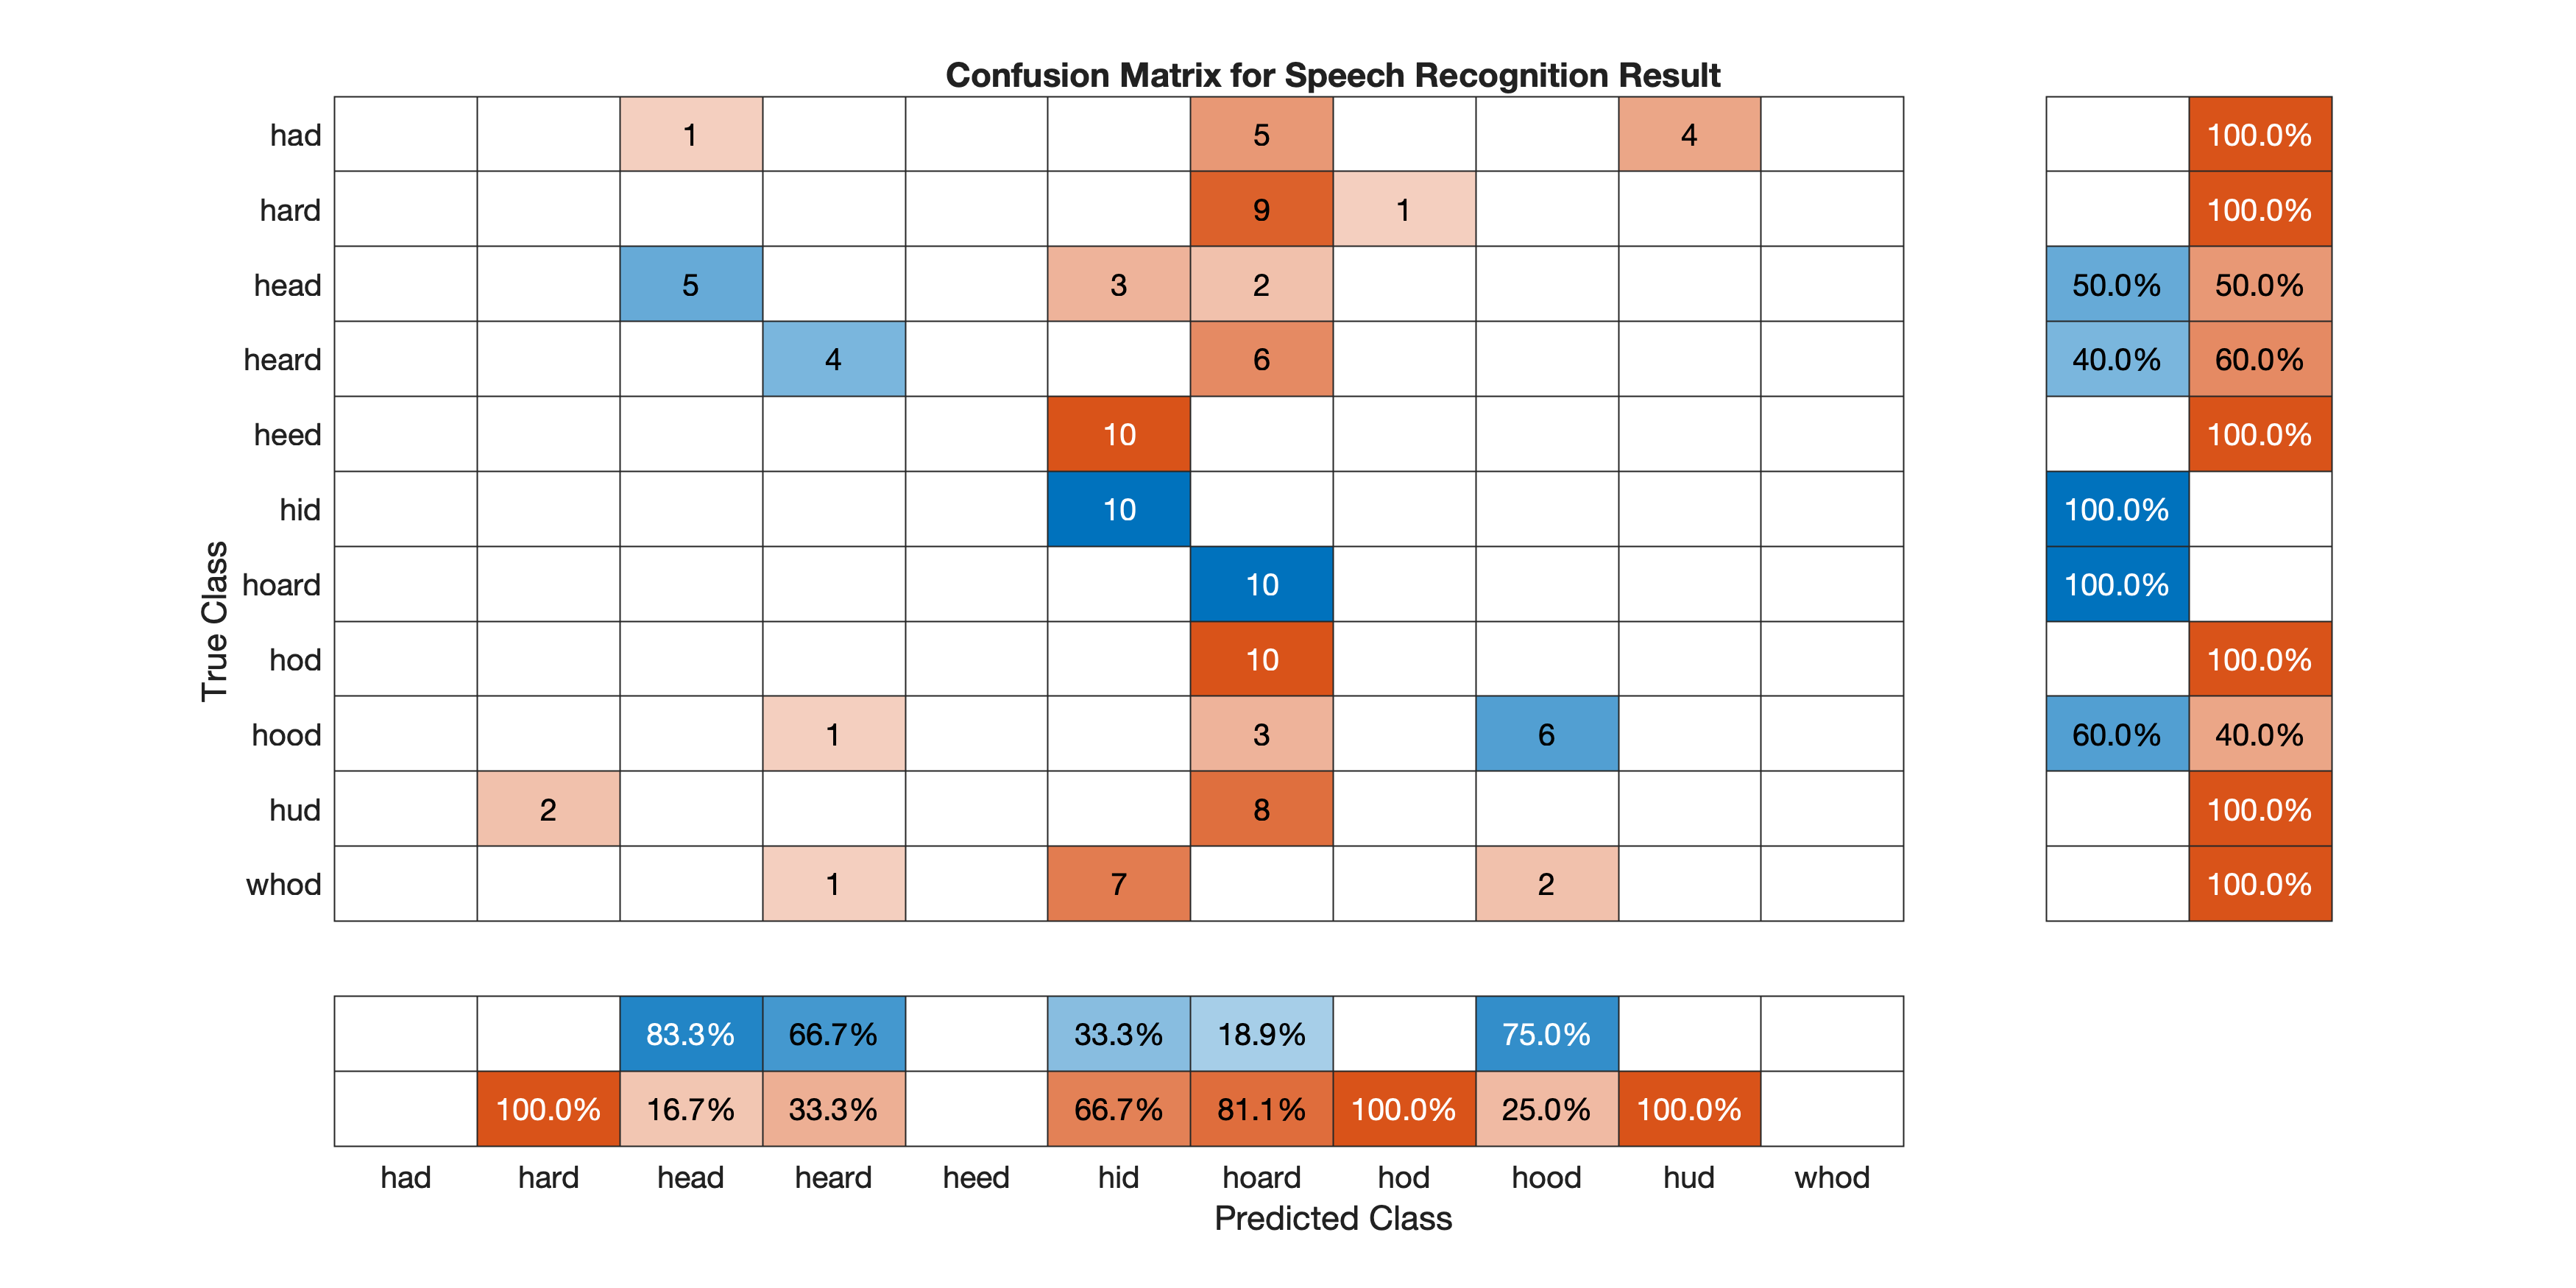
\includegraphics[width=\textwidth]{confusion_matrix}
\end{center}
\caption{\label{fig:confusion-matrix} Confusion matrix for HMM model training on the evaluation set.}
\end{figure}

\section{Data augmentation}

By analyzing the characteristics of the training and validation datasets, as well as the confusion matrix of the predictions on the validation dataset, strategies for optimizing the model’s performance can be developed. The following outlines the optimization of the model’s performance using data augmentation methods.

\paragraph{Characteristics of the validation data:}
The pronunciations in the validation dataset consist entirely of male voices across 11 groups of words.

\paragraph{Evaluation results of the validation data:}
\begin{itemize}
\item The prediction accuracy for "had", "hard", "heed", "hod", "hud" and "whod" is 0%.
\item The prediction accuracy for “hid” and “hoard” is relatively high, at 100\%.	
\end{itemize}

\paragraph{Augmentation measures for the Data:}
\begin{enumerate}
\item Train only on male voices.
\item Perform 3x or 5x repetition augmentation for male voice recordings.
\item Perform 3x or 5x repetition augmentation for audio samples of the words "had", "hard", "heed", "hod", "hud" and "whod".
\end{enumerate}

Following the application of data augmentation techniques, the resulting recognition outputs are evaluated using the optimal HMM model. The associated confusion matrix is presented in Figure \ref{fig:confusion-matrix-augmentation}.

\begin{figure}[!h]
\begin{center}
\includegraphics[width=\textwidth]{confusion_matrix_data_augmentation}
\end{center}
\caption{\label{fig:confusion-matrix-augmentation} Confusion matrix for HMM model training on the data augmentation set.}
\end{figure}

The confusion matrix serves to illustrate that the application of data augmentation in accordance with the specific characteristics of the dataset can result in a notable enhancement of the model's performance. In the future, further speech data augmentation techniques, such as time stretching, time shifting and pitch shifting, can be investigated in order to enhance the results even further.


\section{Conclusion}

The coursework is effective in integrating theoretical concepts with practical applications, illustrating the capabilities and constraints of HMM-based speech recognition on both the provided datasets and user-recorded data. The project offers valuable insights into the effectiveness of maximum likelihood training and its impact on improving recognition accuracy through a detailed analysis of the results.

%%%%%%%%%%%%%%%%%%%%%%%%%%%%%%%%%%%%%%%%%%%%%%%%%%%%%%%%%%%%%%%%%%%%%%%%%%%%%%
% \newpage
\newcommand{\doi}[1]{DOI: \href{http://dx.doi.org/#1}{\nolinkurl{#1}}}
\bibliographystyle{ieeetr}
\bibliography{refs}


%%%%%%%%%%%%%%%%%%%%%%%%%%%%%%%%%%%%%%%%%%%%%%%%%%%%%%%%%%%%%%%%%%%%%%%%%%%%%%
\newpage
\appendix
\section{Appendix: Structure of the codes}

\begin{figure}[h]
\begin{center}
\includegraphics[width=18cm]{codes_structure}
\end{center}
\caption{\label{fig:codes-structure} Structure of the codes.}
\end{figure}

\section{Appendix: Codes}

\begin{lstlisting}[frame=single, numbers=left, style=Matlab-editor, caption={train\_model.m}, label={lst:train_model}]
  %% Author: Xiaoguang Liang (PG/T - Comp Sci & Elec Eng)
%%         Zeyad Abdelmonem (PG/T - Comp Sci & Elec Eng)
%% University of Surrey, United Kingdom
%% Email address: xl01339@surrey.ac.uk
%%                za00632@surrey.ac.uk
%% Time: 22/11/2024 17:44
%%       28/11/2024 15:55
close all;
clear;

% Load train data
trainDataFile = GlobalSetting.TRAIN_DATA;
% trainDataFile = [GlobalSetting.DATA_AUGMENTATION, '/data_augmentation_male_x1.mat'];
% trainDataFile = [GlobalSetting.DATA_AUGMENTATION, '/data_augmentation_male_x2.mat'];
% trainDataFile = [GlobalSetting.DATA_AUGMENTATION, '/data_augmentation_male_x3.mat'];
% trainDataFile = [GlobalSetting.DATA_AUGMENTATION, '/data_augmentation_male_x5.mat'];
% trainDataFile = [GlobalSetting.DATA_AUGMENTATION, '/data_augmentation_male_x10.mat'];
% trainDataFile = [GlobalSetting.DATA_AUGMENTATION, '/data_augmentation_male_x50.mat'];
% trainDataFile = [GlobalSetting.DATA_AUGMENTATION, '/data_augmentation_word_x2.mat'];
% trainDataFile = [GlobalSetting.DATA_AUGMENTATION, '/data_augmentation_word_x5.mat'];
% trainDataFile = [GlobalSetting.DATA_AUGMENTATION, '/data_augmentation_male_word_x5.mat'];
% trainDataFile = [GlobalSetting.DATA_AUGMENTATION, '/data_augmentation_male__x5_female.mat'];
% trainDataFile = [GlobalSetting.DATA_AUGMENTATION, '/data_augmentation_male__x5_word_x3.mat'];
trainData = load(trainDataFile, 'trainData').trainData;
K=size(trainData,2);

% Load test data
testDataFile = GlobalSetting.TEST_DATA;
testData = load(testDataFile, 'testData').testData;
K_test=size(testData,2);

% The state of HMM model
N = GlobalSetting.N;
% Parameter dimension
D = GlobalSetting.D;

WORDS = GlobalSetting.WORDS;
words_len = length(WORDS);

wordData = {trainData.word};

% Calculate MFCCs
disp('Calculating MFCCs...');
for k = 1:K
    if isfield(trainData(k),'data') & ~isempty(trainData(k).data)
        continue;
    else
        sampleData = trainData(k).sampleData;
        sampleRate = trainData(k).sampleRate;
        mfccCoeff = mfccFeature(sampleData, sampleRate, D);
        trainData(k).data = mfccCoeff;
    end
end

% Train HMM model
epochs = GlobalSetting.EPOCHS;
all_errors = zeros(epochs, 1);
hmm_models = struct();
lowest_error = 1;

for loop = 1:epochs
    fprintf('Starting Epoch %d ... \n', loop)
    % Run training with different group data based on different word.
    for i=1:words_len
        word = WORDS{i};
        fprintf('Start training %s group data\n', word);
        % Find the index of word
        idxes = find(strcmp(wordData, word));

        samples = trainData(idxes);
        % The number of pdf in each state
        PDFS = repmat(D, 1, N);
        if loop == 1
            hmm = init_hmm(samples, PDFS);
        else
            % update hmm model
            hmm = hmm_models.(word);
        end
        hmm_models.(word)=Baum_Welch(hmm, samples);
    end

    % Evaluate the model
    v_output(loop)=0;
    for k = 1:K_test
        data = testData(:,k);
        sampleData = data.sampleData;
        sampleRate = data.sampleRate;
        % Compute MFCC coefficients
        mfccCoeff = mfccFeature(sampleData, sampleRate, D);
        for j=1:words_len
            word = WORDS{j};
            hmm = hmm_models.(word);
            [viterbi_res, ~] = viterbi(hmm, mfccCoeff);
            pout(j) = viterbi_res;
            v_output(loop) = v_output(loop) + viterbi_res;
        end
        [d,n] = max(pout);
        word_res = WORDS{n};
        testData(k).prediction = word_res;
    end

    % Compute error rate
    trueSequence = {testData.word};
    predictedSequence = {testData.prediction};
    [errorRate] = compute_error_rate(trueSequence, predictedSequence);
    all_errors(loop) = errorRate;

    fprintf('%d Epoch, The recognition error rate is %f\n', loop, errorRate)

    % Update the best model if current error rate is lower than the best one
    if errorRate <= lowest_error
        lowest_error = errorRate;
        best_hmm = hmm_models;
        fprintf('New best model found: model of loop %d !\n', loop);
    end

    % Convergence monitoring
    % Compare the distance between two HMMs.
    if loop>1
        difference = abs((v_output(loop)-v_output(loop-1))/v_output(loop));
        fprintf('Difference of the viterbi output = %d\n', difference);
        if  difference < 2e-5
            fprintf('The model converges!\n');
            % break
        end
    end

    % Save the HMM model
    saveDir = GlobalSetting.HMM_MODEL;
    if ~exist(saveDir, 'dir')
        % Create the new directory
        mkdir(saveDir);
    end

    str_loop = num2str(loop);
    model_file = [saveDir, '/hmm_models_', str_loop, '.mat'];
    % model_file = strjoin(model_file, '');
    save(model_file, 'hmm_models');

end

% Plot the error rate
epoch_list = 1:epochs;
plot_errors(epoch_list, all_errors);


\end{lstlisting}

\begin{lstlisting}[frame=single, numbers=left, style=Matlab-editor, caption={test\_model.m}, label={lst:test_model}]
  %% Author: Xiaoguang Liang (PG/T - Comp Sci & Elec Eng)
%% University of Surrey, United Kingdom
%% Email address: xl01339@surrey.ac.uk
%% Time: 22/11/2024 23:05

clc;
close all;
clear;

D = 13;

% Load test data
% testDataFile = GlobalSetting.TEST_DATA;
% testData = load(testDataFile, 'testData').testData;

% Load evaluation data
evaluationDataFile = GlobalSetting.EVALUATION_DATA;
evaluationData = load(evaluationDataFile, 'evaluationData').evaluationData;

% Load HMM model
model_num = 11;
model_file = [GlobalSetting.HMM_MODEL, '/hmm_models_', num2str(model_num), '.mat'];
hmm_model = load(model_file, 'hmm_models').hmm_models;
WORDS = GlobalSetting.WORDS;
words_len = length(WORDS);

Ndata = size(evaluationData,2);
% Ndata = size(testData,2);

p = 0;
n = 0;
for i=1:Ndata
    data = evaluationData(:,i);
    sampleData = data.sampleData;
    sampleRate = data.sampleRate;
    true_word = data.word;
    % Compute MFCC coefficients
    mfccCoeff = mfccFeature(sampleData, sampleRate, D);

    % Recognize the word
    for j=1:words_len
        word = WORDS{j};
        hmm = hmm_model.(word);
        pout(j) = viterbi(hmm, mfccCoeff);
    end
    [d,n] = max(pout);

    word_res = WORDS{n};
    evaluationData(i).prediction = word_res;
    fprintf('The NO. %d word is recognized as %s\n', i-1,word_res)
    if strcmp(word_res, true_word)
        p = p+1;
        fprintf('The recognition is correct\n')
    else
        n = n+1;
        fprintf('The recognition is incorrect\n')
    end

end

accuracy = p/Ndata;
fprintf('The recognition rate is %f\n', accuracy)

% Save the recognition result
file = GlobalSetting.RECOGNITION_RESULT;
save(file, 'evaluationData');

\end{lstlisting}

\begin{lstlisting}[frame=single, numbers=left, style=Matlab-editor, caption={compute\_confusion\_matrix.m}, label={lst:compute_confusion_matrix}]
  %% Author: Xiaoguang Liang (PG/T - Comp Sci & Elec Eng)
%% University of Surrey, United Kingdom
%% Email address: xl01339@surrey.ac.uk
%% Time: 03/12/2024 22:19

clc;
close all;
clear;

% Load recognition result
evaluationDataFile = GlobalSetting.RECOGNITION_RESULT;
evaluationData = load(evaluationDataFile, 'evaluationData').evaluationData;


true_word = {evaluationData.word};
prediction = {evaluationData.prediction};

% Plot the confusion matrix
fig = figure;
cm = confusionchart(true_word,prediction, 'RowSummary','row-normalized','ColumnSummary','column-normalized');
cm.Title = 'Confusion Matrix for Speech Recognition Result';

fig_Position = fig.Position;
fig_Position(3) = fig_Position(3)*1.5;
fig.Position = fig_Position;

% Save the graph as a high-resolution PNG file
saveDir = GlobalSetting.GRAPH_PATH;
if ~exist(saveDir, 'dir')
    % Create the new directory
    mkdir(saveDir);
end
savePath=[saveDir, '/confusion_matrix.png'];

% exportgraphics(fig, savePath, 'Resolution', 300);
% Save the figure as a PNG file with specified margins
print(gcf, savePath, '-dpng', '-r300');  % '-r300' sets 300 DPI for high resolution

\end{lstlisting}

\begin{lstlisting}[frame=single, numbers=left, style=Matlab-editor, caption={GlobalSetting.m}, label={lst:GlobalSetting}]
  classdef GlobalSetting
    %GLOBALSETTING Summary of this class goes here
    %   Detailed explanation goes here

    properties(Constant=true)
        % Dataset path
        DATASET_FOLDER = 'data/EEEM030cw2-DevelopmentSet-2024';
        EVALUATION_FOLDER = 'data/EEEM030cw2-EvaluationSet-2024';
        TRAIN_DATA = 'data/trainData.mat';
        TEST_DATA = 'data/testData.mat';
        EVALUATION_DATA = 'data/evaluationData.mat';
        HMM_MODEL = 'data/hmm_models'
        RECOGNITION_RESULT = 'data/recognition_result.mat'
        GRAPH_PATH = 'data/graphs'
        DATA_AUGMENTATION = 'data/data_augmentation'

        % words for speech recognition
        WORDS = {'heed', 'hid', 'head', 'had', 'hard', 'hud', 'hod', 'hoard', 'hood', 'whod', 'heard'}

        % Epochs for training
        EPOCHS = 15

        % HMM parameters
        % The state of HMM model
        N = 8;
        % The dimension of continuous probability density function
        D = 13;

        % Based on the instructions in the assignment, we can get initial A and Pi in Table 1
        A_init = [0.8 0.2 0.0 0.0 0.0 0.0 0.0 0.0,
            0.0 0.8 0.2 0.0 0.0 0.0 0.0 0.0,
            0.0 0.0 0.8 0.2 0.0 0.0 0.0 0.0,
            0.0 0.0 0.0 0.8 0.2 0.0 0.0 0.0,
            0.0 0.0 0.0 0.0 0.8 0.2 0.0 0.0,
            0.0 0.0 0.0 0.0 0.0 0.8 0.2 0.0,
            0.0 0.0 0.0 0.0 0.0 0.0 0.8 0.2,
            0.0 0.0 0.0 0.0 0.0 0.0 0.0 0.8];
        Pi_init = [1.0 0.0 0.0 0.0 0.0 0.0 0.0 0.0];
        eta_init = [0 0 0 0 0 0 0 0.2]';

        % Replace NaNs with 0
        REPLACE_NAN = 0;

    end

    methods
        function obj = GlobalSetting()
            %GLOBALSETTING Construct an instance of this class
            %   Detailed explanation goes here
        end
    end
end


\end{lstlisting}

\begin{lstlisting}[frame=single, numbers=left, style=Matlab-editor, caption={mfccFeature.m}, label={lst:mfccFeature}]
  function mfccCoeff = mfccFeature(sampleData, sampleRate, Dimension)
% MFCCFEATURE Summary of this function goes here
%
% [OUTPUTARGS] = MFCCFEATURE(INPUTARGS) Explain usage here
%
% Examples:
%
% Provide sample usage code here
%
% See also: List related files here

% Author: Tofarati Onatunde, Xiaoguang Liang, University of Surrey
% Date: 2024/11/22 23:26:20
% Revision: 0.1


% PARAMETERS
frame_length_ms = 30;   % Frame length in ms
hop_size_ms = 10;       % Hop size in ms

% Frame size and hop size in samples
frame_length_samples = round(frame_length_ms / 1000 * sampleRate);  % Convert ms to samples
hop_size_samples = round(hop_size_ms / 1000 * sampleRate);        % Convert ms to samples

% Define a function for extracting MFCCs from a windowed frame
extract_mfcc_from_frame = @(audio, fs, frame_length, hop_size, num_coeffs) ...
    mfcc(audio, fs, 'Window', hamming(frame_length, 'periodic'), ...
    'OverlapLength', frame_length - hop_size, 'NumCoeffs', num_coeffs, 'LogEnergy', 'replace');

% Extract MFCCs for each audio file using frame-based processing
mfccCoeff = extract_mfcc_from_frame(sampleData, sampleRate, frame_length_samples, hop_size_samples, Dimension);

end

\end{lstlisting}

\begin{lstlisting}[frame=single, numbers=left, style=Matlab-editor, caption={shared\_feature\_extraction.mlx}, label={lst:shared_feature_extraction}]
  % FEATURE EXTRACTION // FEATURE EXTRACTION // FEATURE EXTRACTION // FEATURE EXTRACTION
% Shared folder

%Note switch these audios to analyse different signals
% one as the training set and another as the test set
[heed, fs_heed] = audioread('sp01a_w01_heed.mp3'); 
[hid, fs_hid]  = audioread('sp01a_w02_hid.mp3');
[head, fs_head]  = audioread('sp01a_w03_head.mp3');
[had, fs_had]  = audioread('sp01a_w04_had.mp3');
[hard, fs_hard]  = audioread('sp01a_w05_hard.mp3');
[hud, fs_hud]  = audioread('sp01a_w06_hud.mp3');
[hod, fs_hod]  = audioread('sp01a_w07_hod.mp3');
[hoard, fs_hoard]  = audioread('sp01a_w08_hoard.mp3');
[hood, fs_hood]  = audioread('sp01a_w09_hood.mp3');
[whod, fs_whod]  = audioread('sp01a_w10_whod.mp3');
[heard, fs_heard]  = audioread('sp01a_w11_heard.mp3');

t1 = (0:length(heed)-1) / fs_heed; 
t2 = (0:length(hid)-1) / fs_hid;  
t3 = (0:length(head)-1) / fs_head; 
t4 = (0:length(had)-1) / fs_had;
t5 = (0:length(hard)-1) / fs_hard; 
t6 = (0:length(hud)-1) / fs_hud;
t7 = (0:length(hod)-1) / fs_hod; 
t8 = (0:length(hoard)-1) / fs_hoard;
t9 = (0:length(hood)-1) / fs_hood; 
t10 = (0:length(whod)-1) / fs_whod;
t11 = (0:length(heard)-1) / fs_heard; 


% PLOT OF SIGNALS
plot(t1, heed);  
axis tight
xlabel('Time (S)');
ylabel('Amplitude');
title('HEED');

plot(t2, hid);  
axis tight
xlabel('Time (S)');
ylabel('Amplitude');
title('HID');

plot(t3, head);  
axis tight
xlabel('Time (S)');
ylabel('Amplitude');
title('HEAD');

plot(t4, had);  
axis tight
xlabel('Time (S)');
ylabel('Amplitude');
title('HAD');
 
plot(t5, hard);  
axis tight
xlabel('Time (S)');
ylabel('Amplitude');
title('HARD');

plot(t6, hud);  
axis tight
xlabel('Time (S)');
ylabel('Amplitude');
title('HUD');

plot(t7, hod);  
axis tight
xlabel('Time (S)');
ylabel('Amplitude');
title('HOD');

plot(t8, hoard);  
axis tight
xlabel('Time (S)');
ylabel('Amplitude');
title('HOARD');

plot(t9, hood);  
axis tight
xlabel('Time (S)');
ylabel('Amplitude');
title('HOOD');

plot(t10, whod);  
axis tight
xlabel('Time (S)');
ylabel('Amplitude');
title('WHOD');

plot(t11, heard);  
axis tight
xlabel('Time (S)');
ylabel('Amplitude');
title('HEARD');



% PARAMETERS
frame_length_ms = 30;   % Frame length in ms
hop_size_ms = 10;       % Hop size in ms
num_mfcc_coeffs = 13;   % Number of MFCC coefficients (including zeroth)

% Frame size and hop size in samples
frame_length_samples = round(frame_length_ms / 1000 * fs_heed);  % Convert ms to samples
hop_size_samples = round(hop_size_ms / 1000 * fs_heed);        % Convert ms to samples

% Define a function for extracting MFCCs from a windowed frame
extract_mfcc_from_frame = @(audio, fs, frame_length, hop_size, num_coeffs) ...
    mfcc(audio, fs, 'Window', hamming(frame_length, 'periodic'), ...
         'OverlapLength', frame_length - hop_size, 'NumCoeffs', num_coeffs);


% Extract MFCCs for each audio file using frame-based processing
mfcc_heed = extract_mfcc_from_frame(heed, fs_heed, frame_length_samples, hop_size_samples, num_mfcc_coeffs);
mfcc_hid = extract_mfcc_from_frame(hid, fs_hid, frame_length_samples, hop_size_samples, num_mfcc_coeffs);
mfcc_head = extract_mfcc_from_frame(head, fs_head, frame_length_samples, hop_size_samples, num_mfcc_coeffs);
mfcc_had = extract_mfcc_from_frame(had, fs_had, frame_length_samples, hop_size_samples, num_mfcc_coeffs);
mfcc_hard = extract_mfcc_from_frame(hard, fs_hard, frame_length_samples, hop_size_samples, num_mfcc_coeffs);
mfcc_hud = extract_mfcc_from_frame(hud, fs_hud, frame_length_samples, hop_size_samples, num_mfcc_coeffs);
mfcc_hod = extract_mfcc_from_frame(hod, fs_hod, frame_length_samples, hop_size_samples, num_mfcc_coeffs);
mfcc_hoard = extract_mfcc_from_frame(hoard, fs_hoard, frame_length_samples, hop_size_samples, num_mfcc_coeffs);
mfcc_hood = extract_mfcc_from_frame(hood, fs_hood, frame_length_samples, hop_size_samples, num_mfcc_coeffs);
mfcc_whod = extract_mfcc_from_frame(whod, fs_whod, frame_length_samples, hop_size_samples, num_mfcc_coeffs);
mfcc_heard = extract_mfcc_from_frame(heard, fs_heard, frame_length_samples, hop_size_samples, num_mfcc_coeffs);

% DISPLAY THE MFCCs
disp('MFCC for "heed":');
disp(mfcc_heed);

disp('MFCC for "hid":');
disp(mfcc_hid);

disp('MFCC for "head":');
disp(mfcc_heed);

disp('MFCC for "hid":');
disp(mfcc_hid);

disp('MFCC for "hard":');
disp(mfcc_hard);

disp('MFCC for "hud":');
disp(mfcc_hud);

disp('MFCC for "hod":');
disp(mfcc_hod);

disp('MFCC for "hoard":');
disp(mfcc_hoard);

disp('MFCC for "hood":');
disp(mfcc_hood);

disp('MFCC for "whod":');
disp(mfcc_whod);

disp('MFCC for "heard":');
disp(mfcc_heard);


% DISPLAY OF THE MFCC OF THE AUDIO SIGNALS - SPECTOGRAM
imagesc(mfcc_heed');  % Transpose to display the frames on the x-axis
colorbar;
xlabel('Frame');
ylabel('MFCC Coefficients');
title('MFCCs for "heed"');

imagesc(mfcc_hid');  
colorbar;
xlabel('Frame');
ylabel('MFCC Coefficients');
title('MFCCs for "hid"');

imagesc(mfcc_head');  
colorbar;
xlabel('Frame');
ylabel('MFCC Coefficients');
title('MFCCs for "head"');

imagesc(mfcc_had'); 
colorbar;
xlabel('Frame');
ylabel('MFCC Coefficients');
title('MFCCs for "had"');

imagesc(mfcc_hard'); 
colorbar;
xlabel('Frame');
ylabel('MFCC Coefficients');
title('MFCCs for "hard"');

imagesc(mfcc_hud'); 
colorbar;
xlabel('Frame');
ylabel('MFCC Coefficients');
title('MFCCs for "hud"');

imagesc(mfcc_hod'); 
colorbar;
xlabel('Frame');
ylabel('MFCC Coefficients');
title('MFCCs for "hod"');

imagesc(mfcc_hoard');  
colorbar;
xlabel('Frame');
ylabel('MFCC Coefficients');
title('MFCCs for "hoard"');

imagesc(mfcc_hood');  
colorbar;
xlabel('Frame');
ylabel('MFCC Coefficients');
title('MFCCs for "hood"');

imagesc(mfcc_whod'); 
colorbar;
xlabel('Frame');
ylabel('MFCC Coefficients');
title('MFCCs for "whod"');

imagesc(mfcc_heard');  
colorbar;
xlabel('Frame');
ylabel('MFCC Coefficients');
title('MFCCs for "heard"');


% PLAY THE AUDIOS WITH THEIR CORRESPONDING SAMPLE RATES
sound(heed, fs_heed);  % Play 'heed'
pause(length(heed)/fs_heed);
sound(hid, fs_hid);  % Play 'hid'
pause(length(hid)/fs_hid); 
sound(head, fs_head); % PLay 'head'
pause(length(head)/fs_head);  
sound(had, fs_had);  % Play 'had'
pause(length(had)/fs_had);
sound(hard, fs_hard);  % Play 'hard'
pause(length(hard)/fs_hard);
sound(hud, fs_hud);  % Play 'hud'
pause(length(hud)/fs_hud);
sound(hod, fs_hod);  % Play 'hod'
pause(length(hod)/fs_hod);
sound(hoard, fs_hoard);  % Play 'hoard'
pause(length(hoard)/fs_hoard);
sound(hood, fs_hood);  % Play 'hood'
pause(length(hood)/fs_hood);
sound(whod, fs_whod);  % Play 'whod'
pause(length(whod)/fs_whod);
sound(heard, fs_heard);  % Play 'heard'
pause(length(heard)/fs_heard);

\end{lstlisting}

\begin{lstlisting}[frame=single, numbers=left, style=Matlab-editor, caption={Baum\_Welch.m}, label={lst:Baum_Welch}]
  function [hmm] = Baum_Welch(hmm, samples)
% BAUM_WELCH Summary of this function goes here
%
% [OUTPUTARGS] = BAUM_WELCH(INPUTARGS) Explain usage here
%
% Examples:
%
% Provide sample usage code here
%
% See also: List related files here

% Author: Xiaoguang Liang, University of Surrey
% Date: 2024/12/03 00:11:46
% Revision: 0.1

% Gaussian Mixture states
mix = hmm.mix;
% HMM states
N = length(mix);
% Number of samples
K = length(samples);
% Parameter dimension
DIM = GlobalSetting.D;

% Accumulate the Forward and Backward Likelihoods and  Occupation Likelihoods.
for k = 1:K
    likelihoods(k) = obtain_likelihoods(hmm, samples(k).data);
end

% Re-estimate transition probability matrix A 
disp('Re-estimate transition probability matrix A...')
for i = 1:N-1
    denom = 0;
    for k = 1:K
        tmp   = likelihoods(k).ksai(:,i,:);
        denom = denom + sum(tmp(:));
    end
    for j = i:i+1
        nom = 0;
        for k = 1:K
            tmp = likelihoods(k).ksai(:,i,j);
            nom = nom   + sum(tmp(:));
        end
        hmm.trans(i,j) = nom / denom;
    end
end


% Avoid getting NaN
hmm.trans(isnan(hmm.trans))=GlobalSetting.REPLACE_NAN;

% Re-estimate the parameters of Gaussian mixture
disp('Re-estimate the parameters of Gaussian mixture...')
for l = 1:N
    for j = 1:hmm.M(l)
        % Compute mean and variance of pdf
        nommean = zeros(1,DIM);
        nomvar  = zeros(1,DIM);
        denom   = 0;
        for k = 1:K
            T = size(samples(k).data,1);
            for t = 1:T
                x = samples(k).data(t,:);
                nommean = nommean + likelihoods(k).gama(t,l,j) * x;
                nomvar  = nomvar  + likelihoods(k).gama(t,l,j) * (x-mix(l).mean(j,:)).^2;
                denom   = denom   + likelihoods(k).gama(t,l,j);
            end
        end
        hmm.mix(l).mean(j,:) = nommean / denom;
        hmm.mix(l).var (j,:) = nomvar  / denom;

        % Compute the weight of pdf
        nom   = 0;
        denom = 0;
        for k = 1:K
            tmp = likelihoods(k).gama(:,l,j);
            nom = nom + sum(tmp(:));
            tmp = likelihoods(k).gama(:,l,:);
            denom = denom + sum(tmp(:));
        end
        % Avoid that weight is NaN
        if denom==0, weight=GlobalSetting.REPLACE_NAN; end
        weight = nom/denom;
        % Avoid probabilities smaller than realmin
        weight = max(weight, realmin); 
        hmm.mix(l).weight(j) = weight;
    end
end

\end{lstlisting}

\begin{lstlisting}[frame=single, numbers=left, style=Matlab-editor, caption={compute\_backward\_likelihood.m}, label={lst:compute_backward_likelihood}]
  function [beta] = compute_backward_likelihood(T, N, c, mix, trans, observations)
% COMPUTE_BACKWARD_LIKELIHOOD Summary of this function goes here
% 
% [OUTPUTARGS] = COMPUTE_BACKWARD_LIKELIHOOD(INPUTARGS) Explain usage here
% 
% Examples: 
% 
% Provide sample usage code here
% 
% See also: List related files here

% Author: Xiaoguang Liang, University of Surrey 
% Date: 2024/12/04 10:36:16 
% Revision: 0.1 

% Given the observation sequence O, calculate the backward probabilities beta.
beta = zeros(T,N);

% The backward probability at t = T and its normalization.
for l = 1:N
    beta(T,l) = c(T);
end

% The backward probabilities from t = T -1 to t = 1 and their normalization.
for t = T-1:-1:1
    x = observations(t+1,:);
    for i = 1:N
    	for j = 1:N
    		beta(t,i) = beta(t,i) + beta(t+1,j) * compute_probability(mix(j),x) * trans(i,j);
    	end
    end
    beta(t,:) = c(t) * beta(t,:);
    % Scale the backward probabilities
    beta(t,:) = beta(t,:)/sum( beta(t,:));
end

% Avoid getting NaN
beta(isnan(beta))=GlobalSetting.REPLACE_NAN;
end

\end{lstlisting}

\begin{lstlisting}[frame=single, numbers=left, style=Matlab-editor, caption={compute\_error\_rate.m}, label={lst:compute_error_rate}]
  function [errorRate] = compute_error_rate(trueSequence, predictedSequence)
% COMPUTE_ERROR_RATE Summary of this function goes here
% 
% [OUTPUTARGS] = COMPUTE_ERROR_RATE(INPUTARGS) Explain usage here
% 
% Examples: 
% 
% Provide sample usage code here
% 
% See also: List related files here

% Author: Xiaoguang Liang, University of Surrey 
% Date: 2024/12/04 20:56:48 
% Revision: 0.1 

% Calculate the number of mismatches
% Ensure the two cells are of the same size
if length(trueSequence) ~= length(predictedSequence)
  error('The two cells must have the same length for comparison.');
end

% Initialize mismatch counter
numErrors = 0;

% Loop through each element to compare
for i = 1:length(trueSequence)
  if ~strcmp(trueSequence{i}, predictedSequence{i})
    numErrors = numErrors + 1;
  end
end

% Calculate the total number of observations
totalObservations = length(trueSequence);

% Calculate error rate
errorRate = numErrors / totalObservations;

end

\end{lstlisting}

\begin{lstlisting}[frame=single, numbers=left, style=Matlab-editor, caption={compute\_forward\_likelihood.m}, label={lst:compute_forward_likelihood}]
  function [alpha, c] = compute_forward_likelihood(T, N, init, mix, trans, observations)
% COMPUTE_FORWARD_LIKELIHOOD Summary of this function goes here
% 
% [OUTPUTARGS] = COMPUTE_FORWARD_LIKELIHOOD(INPUTARGS) Explain usage here
% 
% Examples: 
% 
% Provide sample usage code here
% 
% See also: List related files here

% Author: Xiaoguang Liang, University of Surrey 
% Date: 2024/12/04 10:36:02 
% Revision: 0.1 

% Given the observation sequence, calculate the forward probability.
alpha = zeros(T,N);

% The forward probability at t = 1.
x = observations(1,:);
for i = 1:N
    alpha(1,i) = init(i) * compute_probability(mix(i),x);
end

% Initialize the forward probability for t = 1.
c    = zeros(T,1);
c(1) = 1/sum(alpha(1,:));
alpha(1,:) = c(1) * alpha(1,:);

% The forward probabilities and initialization for t = 2 to T.
for t = 2:T
    for i = 1:N
        temp = 0;
        for j = 1:N
            temp = temp + alpha(t-1,j) * trans(j,i);
        end
        alpha(t,i) = temp * compute_probability(mix(i),observations(t,:));
    end
    % Scale the forward probabilities.
    c(t) = 1/sum(alpha(t,:));
    alpha(t,:) = c(t)*alpha(t,:);
end

% Avoid getting NaN
c(isnan(c))=GlobalSetting.REPLACE_NAN;
alpha(isnan(alpha))=GlobalSetting.REPLACE_NAN;
end

\end{lstlisting}

\begin{lstlisting}[frame=single, numbers=left, style=Matlab-editor, caption={compute\_occupation\_likelihood.m}, label={lst:compute_occupation_likelihood}]
  function [gama] = compute_occupation_likelihood(T, N, mix, hmm, observations, alpha, beta)
% COMPUTE_OCCUPATION_LIKELIHOOD Summary of this function goes here
% 
% [OUTPUTARGS] = COMPUTE_OCCUPATION_LIKELIHOOD(INPUTARGS) Explain usage here
% 
% Examples: 
% 
% Provide sample usage code here
% 
% See also: List related files here

% Author: Xiaoguang Liang, University of Surrey 
% Date: 2024/12/04 10:36:37 
% Revision: 0.1 

% The mixture output probability: gama, i.e B.
gama = zeros(T,N,max(hmm.M));
for t = 1:T
    pab = zeros(N,1);
    for l = 1:N
        pab(l) = alpha(t,l) * beta(t,l);
    end
    x = observations(t,:);
    for l = 1:N
        prob = zeros(mix(l).M,1);
        for j = 1:mix(l).M
            m = mix(l).mean(j,:);
            v = mix(l).var (j,:);
            prob(j) = mix(l).weight(j) * compute_pdf(m, v, x);
        end
        tmp  = pab(l)/sum(pab);
        for j = 1:mix(l).M
            gama(t,l,j) = tmp * prob(j)/sum(prob);
        end
    end
end

% Avoid getting NaN
gama(isnan(gama))=GlobalSetting.REPLACE_NAN;
end

\end{lstlisting}

\begin{lstlisting}[frame=single, numbers=left, style=Matlab-editor, caption={compute\_pdf\_gm.m}, label={lst:compute_pdf_gm}]
  function [p] = compute_pdf_gm(m, v, x)
% GET_PDF Summary of this function goes here
%
% [OUTPUTARGS] = GET_PDF(INPUTARGS) Explain usage here
%
% Examples:
%
% Provide sample usage code here
%
% See also: List related files here

% Author: Xiaoguang Liang, University of Surrey
% Date: 2024/12/03 00:35:32
% Revision: 0.1

% Regularization to prevent zero variances
epsilon = 1e-8; % Small value to prevent numerical instability
v = v + epsilon;

% Dimension of the data
D = length(v);

% Check for consistency in dimensions
if length(m) ~= D || length(x) ~= D
    error('Mean, variance, and data point must have the same dimension.');
end

% Normalization factor
norm_factor = (2 * pi) ^ (-D / 2) * prod(v .^ -0.5);

% Compute the exponent
diff = x - m;
exponent = -0.5 * sum((diff .^ 2) ./ v);

% Avoid overflow/underflow in exponential
exponent = max(exponent, -700); % Prevent exp(-inf) (numerical limit of exp in MATLAB)

% Compute the probability
p = norm_factor * exp(exponent);

% Avoid probabilities smaller than realmin
p = max(p, realmin);

% Avoid getting NaN
if isnan(p), p=GlobalSetting.REPLACE_NAN; end

end

\end{lstlisting}

\begin{lstlisting}[frame=single, numbers=left, style=Matlab-editor, caption={compute\_pdf.m}, label={lst:compute_pdf}]
  function [p] = compute_pdf(m, v, x)
% GET_PDF Summary of this function goes here
%
% [OUTPUTARGS] = GET_PDF(INPUTARGS) Explain usage here
%
% Examples:
%
% Provide sample usage code here
%
% See also: List related files here

% Author: Xiaoguang Liang, University of Surrey
% Date: 2024/12/03 00:35:32
% Revision: 0.1

p = (2 * pi * prod(v)) ^ -0.5 * exp(-0.5 * (x-m) ./ v * (x-m)');

% Avoid getting NaN
if isnan(p), p=GlobalSetting.REPLACE_NAN; end

end

\end{lstlisting}

\begin{lstlisting}[frame=single, numbers=left, style=Matlab-editor, caption={compute\_probability.m}, label={lst:compute_probability}]
  function [prob] = compute_probability(mix, x)
% MIXTURE Summary of this function goes here
%
% [OUTPUTARGS] = MIXTURE(INPUTARGS) Explain usage here
%
% Examples:
%
% Provide sample usage code here
%
% See also: List related files here

% Author: Xiaoguang Liang, University of Surrey
% Date: 2024/12/03 00:30:05
% Revision: 0.1

prob = 0;
for j = 1:mix.M
    m = mix.mean(j,:);
    v = mix.var (j,:);
    w = mix.weight(j);
    % pdf = compute_pdf(m, v, x);
    pdf = compute_pdf_gm(m, v, x);
    prob = prob + w * pdf;
end

% Add realmin to prevent overflow when calculating log(prob) in viterbi.m.
if prob==0, prob=realmin; end

\end{lstlisting}

\begin{lstlisting}[frame=single, numbers=left, style=Matlab-editor, caption={compute\_transition\_likelihood.m}, label={lst:compute_transition_likelihood}]
  function [ksai] = compute_transition_likelihood(T, N, c, mix, trans, observations, alpha, beta)
% COMPUTE_TRANSITION_LIKELIHOOD Summary of this function goes here
% 
% [OUTPUTARGS] = COMPUTE_TRANSITION_LIKELIHOOD(INPUTARGS) Explain usage here
% 
% Examples: 
% 
% Provide sample usage code here
% 
% See also: List related files here

% Author: Xiaoguang Liang, University of Surrey 
% Date: 2024/12/04 10:37:05 
% Revision: 0.1 

% The transition probability ksai, i.e. A.
ksai = zeros(T-1,N,N);
for t = 1:T-1
    denom = sum(alpha(t,:).*beta(t,:));
    for i = 1:N-1
    	for j = i:i+1
    		nom = alpha(t,i) * trans(i,j) * compute_probability(mix(j),observations(t+1,:)) * beta(t+1,j);
    		ksai(t,i,j) = c(t) * nom/denom;
    	end
    end
end

% Avoid getting NaN
ksai(isnan(ksai))=GlobalSetting.REPLACE_NAN;
end

\end{lstlisting}

\begin{lstlisting}[frame=single, numbers=left, style=Matlab-editor, caption={obtain\_likelihoods.m}, label={lst:obtain_likelihoods}]
  function [likelihoods] = obtain_likelihoods(hmm, observations)
% GET_PARAM Summary of this function goes here
%
% [OUTPUTARGS] = GET_PARAM(INPUTARGS) Explain usage here
%
% Examples:
%
% Provide sample usage code here
%
% See also: List related files here

% Author: Xiaoguang Liang, University of Surrey
% Date: 2024/12/03 00:33:41
% Revision: 0.1

% The length of sequence
T = size(observations,1);
% Initial Pi
init  = hmm.init;
% Initial A
trans = hmm.trans;
% Gaussian Mixture states
mix   = hmm.mix;
% HMM states
N     = hmm.N;

% Given the observation sequence, calculate the forward probability.
[alpha, c] = compute_forward_likelihood(T, N, init, mix, trans, observations);

% Given the observation sequence O, calculate the backward probabilities beta.
[beta] = compute_backward_likelihood(T, N, c, mix, trans, observations);

% The transition probability ksai, i.e. A.
[ksai] = compute_transition_likelihood(T, N, c, mix, trans, observations, alpha, beta);

% The mixture output probability: gama, i.e B.
[gama] = compute_occupation_likelihood(T, N, mix, hmm, observations, alpha, beta);

likelihoods.c     = c;
likelihoods.alpha = alpha;
likelihoods.beta  = beta;
likelihoods.ksai  = ksai;
likelihoods.gama  = gama;


\end{lstlisting}

\begin{lstlisting}[frame=single, numbers=left, style=Matlab-editor, caption={plot\_errors.m}, label={lst:plot_errors}]
  function plot_errors(epochs, errors)
% PLOT_ERRORS Summary of this function goes here
%
% [OUTPUTARGS] = PLOT_ERRORS(INPUTARGS) Explain usage here
%
% Examples:
%
% Provide sample usage code here
%
% See also: List related files here

% Author: Xiaoguang Liang, University of Surrey
% Date: 2024/12/04 19:55:11
% Revision: 0.1

% Adjust the axes position for margins
figure('Position', [100 100 800 500], 'Visible', 'off');

% Get current axes
ax = gca;
% Position: [left, bottom, width, height]
ax.Position = [0.1, 0.1, 0.8, 0.8];

% Set the paper position mode
set(gcf, 'PaperPositionMode', 'auto');

% Set the font format of axis
set(gca, 'Fontname', 'Times New Roman', 'Fontsize', 10);

% Plot the amplitude spectrum of the original segment
plot(epochs, errors, "Color", "#8C92AC", 'LineWidth',2);

xlabel('Epoch');
ylabel('Error rate');

hold on;

% Plot the formant frequencies points
sz = 10;
scatter(epochs, errors, sz, "filled", "o", "MarkerFaceColor", "b");

titleStr = 'Error rate trend for the HMM model';
title(titleStr, 'FontSize', 12);

legend('Error rate curve', 'Error rate points');

% Set the scale
Xmin=1;
Xmax=16;
Ymin=0;
Ymax=1;

% Set maximum and minmum of X and Y
axis([Xmin,Xmax,Ymin,Ymax]);

% Set axis label 
set(gca,'XTick',(Xmin:1:Xmax));
set(gca,'YTick',(Ymin:0.2:Ymax));
set(gca,'LooseInset',get(gca,'TightInset'));
box off;
hold off;

% Save graph
graphName = "Error_rate_trend_for_HMM_model";

saveDir = [GlobalSetting.GRAPH_PATH];
if ~exist(saveDir, 'dir')
    % Create the new directory
    mkdir(saveDir);
end

savePath = [saveDir, '/', graphName, '.png'];
savePath = strjoin(savePath, '');

% Save the figure as a PNG file with specified margins
print(gcf, savePath, '-dpng', '-r300');  % '-r300' sets 300 DPI for high resolution


% Close the invisible figure
close(figure);

end

\end{lstlisting}

\begin{lstlisting}[frame=single, numbers=left, style=Matlab-editor, caption={viterbi.m}, label={lst:viterbi}]
  function [p, q] = viterbi(hmm, O)
% VITERBI Summary of this function goes here
%
% [OUTPUTARGS] = VITERBI(INPUTARGS) Explain usage here
%
% Examples:
%
% Provide sample usage code here
%
% See also: List related files here

% Author: Xiaoguang Liang, Jaison Baptist Sequira, University of Surrey
% Date: 2024/12/03 00:15:17
% Revision: 0.1

% Inital Pi
init  = hmm.init;
% Initial A
trans = hmm.trans;
% Gussian mix
mix = hmm.mix;
% HMM states
N = hmm.N;
% The number of samples
T = size(O,1);

% Process all the parameters with log scale

% Compute log(init)
ind1 = find(init>0);
ind0 = find(init<=0);
init(ind0) = -inf;
init(ind1) = log(init(ind1));

% Compute log(trans)
ind1 = find(trans>0);
ind0 = find(trans<=0);
trans(ind0) = -inf;
trans(ind1) = log(trans(ind1));

% Initialize
delta = zeros(T,N);
phi   = zeros(T,N);
q     = zeros(T,1);

% t=1
x = O(1,:);
for i = 1:N
    delta(1,i) = init(i) + log(compute_probability(mix(i),x));
end

% t=2:T
for t = 2:T
    for j = 1:N
        [delta(t,j) phi(t,j)] = max(delta(t-1,:) + trans(:,j)');
        x = O(t,:);
        delta(t,j) = delta(t,j) + log(compute_probability(mix(j),x));
    end
end

% The final value and the last node
[p, q(T)] = max(delta(T,:));

% Backtrack the best state path.
for t=T-1:-1:1
    q(t) = phi(t+1,q(t+1));
end


end


\end{lstlisting}

\begin{lstlisting}[frame=single, numbers=left, style=Matlab-editor, caption={Gussian\_mix.m}, label={lst:Gussian_mix}]
  function [mix] = Gussian_mix(vector, M, nn)
% GUSSIAN_MIX Summary of this function goes here
%
% [OUTPUTARGS] = GUSSIAN_MIX(INPUTARGS) Explain usage here
%
% Examples:
%
% Provide sample usage code here
%
% See also: List related files here

% Author: Xiaoguang Liang, University of Surrey
% Date: 2024/12/03 19:56:54
% Revision: 0.1

[mean, var] = meanVariance(vector');
mean = mean';
var = var';

% Calculate the number of elements in each cluster and normalize them to obtain the weights for each PDF.
weight = zeros(M,1);
for j = 1:M
    weight(j) = sum(find(j==nn));
end
weight = weight/sum(weight);

% Save the results.
mix.M      = M;
mix.mean   = mean;
mix.var    = var;
mix.weight = weight;

end

\end{lstlisting}

\begin{lstlisting}[frame=single, numbers=left, style=Matlab-editor, caption={init\_hmm.m}, label={lst:init_hmm}]
  function [hmm] = init_hmm(samples, M)
% INIT_HMM Summary of this function goes here
%
% [OUTPUTARGS] = INIT_HMM(INPUTARGS) Explain usage here
%
% Examples:
%
% Provide sample usage code here
%
% See also: List related files here

% Author: Xiaoguang Liang, University of Surrey
% Date: 2024/12/03 00:08:58
% Revision: 0.1

% The number of samples
K = length(samples);
% The number of states
N = length(M);
hmm.N = N;
hmm.M = M;

% Initial state probabilities
hmm.init = GlobalSetting.Pi_init;

% Transition probabilities A
hmm.trans = GlobalSetting.A_init;

% Make N segements
for k = 1:K
    T = size(samples(k).data,1);
    samples(k).segment=floor([1:T/N:T T+1]);
end

% Obtain a continuous Gaussian mixture distribution.
for i = 1:N
    % Combine vectors with the same cluster and the same state into a single vector.
    vector = [];
    nn = [];
    for k = 1:K
        seg1 = samples(k).segment(i);
        seg2 = samples(k).segment(i+1)-1;
        segment_data = samples(k).data(seg1:seg2,:);
        tmp_nn = repmat(k,1,size(segment_data,1))';
        nn = [nn ; tmp_nn];
        vector = [vector ; segment_data];
    end
    mix(i) = Gussian_mix(vector, M(i), nn);
end

hmm.mix = mix;

\end{lstlisting}

\begin{lstlisting}[frame=single, numbers=left, style=Matlab-editor, caption={meanVariance.m}, label={lst:meanVariance}]
  function [meanData, varianceData] = meanVariance(mfccCoeff)
% MEANVARIANCE Calculate the mean and variance of MFCC coefficients.
%
% [MEANDATA, VARIANCEDATA] = MEANVARIANCE(MFCCCOEFF) computes the mean and variance
% of the input MFCC coefficients matrix. The input matrix has dimensions D x M,
% where D is the number of MFCC coefficients and M is the number of observations.
% The function returns two matrices, MEANDATA and VARIANCEDATA, each of size D x D,
% containing the mean and variance values, respectively.
%
% Examples:
%   mfccCoeff = rand(13, 100); % Example MFCC coefficients matrix (13 coefficients, 100 observations)
%   [meanData, varianceData] = meanVariance(mfccCoeff);
%   disp(meanData);
%   disp(varianceData);
%
% See also: mfcc, featureExtraction

% Author: Xiaoguang Liang, University of Surrey
% Date: 2024/11/22 23:28:41
% Revision: 0.1

% Get the dimensions of the input MFCC coefficients matrix
[D, M] = size(mfccCoeff);  % M : number of observations

% Initialize the mean and variance data matrices
meanData = zeros(D, D);
varianceData = zeros(D, D);

% Calculate the number of observations per segment
k = floor(M / D);

% Loop through each segment to calculate the mean and variance
for i = 1:D-1
    % Calculate the mean and variance for the current segment
    meanData(:, i) = mean(mfccCoeff(:, k * (i - 1) + 1:i * k), 2);
    varianceData(:, i) = var(mfccCoeff(:, k * (i - 1) + 1:i * k), 0, 2);
end

% Handle the last segment, which may have fewer observations
i = D;
meanData(:, i) = mean(mfccCoeff(:, k * (i - 1) + 1:end), 2);
varianceData(:, i) = var(mfccCoeff(:, k * (i - 1) + 1:end), 0, 2);

% Normalize the mean and variance
meanData = normalizeMatrix(meanData);
varianceData = normalizeMatrix(varianceData);

% Regulate the variance
% Regularization parameter
epsilon = 1e-8;
varianceData = regularizeCovariance(varianceData, epsilon);

end
\end{lstlisting}

\begin{lstlisting}[frame=single, numbers=left, style=Matlab-editor, caption={normalizeMatrix.m}, label={lst:normalizeMatrix}]
  function normalizedMatrix = normalizeMatrix(matrix, method)
% NORMALIZEMATRIX Summary of this function goes here
%
% [OUTPUTARGS] = NORMALIZEMATRIX(INPUTARGS) Explain usage here
%
% Examples:
%
% Provide sample usage code here
%
% See also: List related files here

% Author: Xiaoguang Liang, University of Surrey
% Date: 2024/12/05 19:01:05
% Revision: 0.1

% Default method if none is provided
if nargin < 2
    method = 'minmax';
end

switch lower(method)
    case 'minmax'
        % Min-max normalization: scale values to [0, 1]
        minVal = min(matrix(:));
        maxVal = max(matrix(:));
        if maxVal == minVal
            warning('Matrix has no variation. Returning zero matrix.');
            normalizedMatrix = zeros(size(matrix));
        else
            normalizedMatrix = (matrix - minVal) / (maxVal - minVal);
        end

    case 'zscore'
        % Z-score normalization: mean = 0, standard deviation = 1
        meanVal = mean(matrix(:));
        stdVal = std(matrix(:));
        if stdVal == 0
            warning('Matrix has no variation. Returning zero matrix.');
            normalizedMatrix = zeros(size(matrix));
        else
            normalizedMatrix = (matrix - meanVal) / stdVal;
        end

    otherwise
        error('Unsupported normalization method. Use ''minmax'' or ''zscore''.');
end
end

\end{lstlisting}

\begin{lstlisting}[frame=single, numbers=left, style=Matlab-editor, caption={regularizeCovariance.m}, label={lst:regularizeCovariance}]
  function regularizedCov = regularizeCovariance(covMatrix, epsilon)
% REGULARIZECOVARIANCE Summary of this function goes here
%
% [OUTPUTARGS] = REGULARIZECOVARIANCE(INPUTARGS) Explain usage here
%
% Examples:
%
% Provide sample usage code here
%
% See also: List related files here

% Author: Xiaoguang Liang, University of Surrey
% Date: 2024/12/05 19:02:12
% Revision: 0.1

% Validate inputs
if ~ismatrix(covMatrix) || size(covMatrix, 1) ~= size(covMatrix, 2)
    error('Input must be a square covariance matrix.');
end

if epsilon <= 0
    error('Regularization term epsilon must be a positive scalar.');
end

% Add epsilon to the diagonal elements
regularizedCov = covMatrix + epsilon * eye(size(covMatrix));

% Ensure symmetry (numerical stability)
regularizedCov = (regularizedCov + regularizedCov') / 2;
end

\end{lstlisting}

\begin{lstlisting}[frame=single, numbers=left, style=Matlab-editor, caption={data\_augmentation.m}, label={lst:data_augmentation}]
  %% Author: Xiaoguang Liang (PG/T - Comp Sci & Elec Eng)
%% University of Surrey, United Kingdom
%% Email address: xl01339@surrey.ac.uk
%% Time: 04/12/2024 17:12

clc;
close all;
clear;

% Characteristics and Evaluation Results of Validation Data:
%
% Characteristics of Validation Data:
% The pronunciations in the validation dataset consist entirely of male voices across 11 groups of words.
%
% Evaluation Results of Validation Data:
% 	•	The prediction accuracy for “had” and “hard” is 0%.
% 	•	The prediction accuracy for “heard” and “whod” is 10%.
% 	•	The prediction accuracy for “hid” and “hoard” is relatively high, at 90% and 100%, respectively.
%
% Enhancement Measures for the Data:
% 	1.	Train only on male voices.
% 	2.	Perform 2x or 3x repetition augmentation for male voice recordings.
% 	3.	Perform 2x or 3x repetition augmentation for audio samples of the words “had,” “hard,” “heard,” and “whod.”

% Male voice prefixes
manPrefix = {'sp01a', 'sp03a', 'sp05a', 'sp07a', 'sp11a', 'sp13a', 'sp14a', 'sp15a', 'sp17a', 'sp22a', 'sp24a', 'sp26a', 'sp28a', 'sp30a'};
womanPrefix = {'sp02a', 'sp04a', 'sp06a', 'sp08a', 'sp09a', 'sp10a', 'sp12a', 'sp16a', 'sp18a', 'sp19a', 'sp20a', 'sp23a', 'sp25a', 'sp27a', 'sp29a'};
childPrefix = {'sp21a'};


% Set the train ratio
trainRatio = 1;

manPrefixLen = length(manPrefix);
numManTrain = round(trainRatio*manPrefixLen);
randManIndex = randperm(manPrefixLen);
trainManPrefix = manPrefix(randManIndex(1:numManTrain));

% womanPrefixLen = length(womanPrefix);
% numWomanTrain = round(trainRatio*womanPrefixLen);
% randWomanIndex = randperm(womanPrefixLen);
% trainWomanPrefix = womanPrefix(randWomanIndex(1:numWomanTrain));

% Get all the audio files
datasetFolder = GlobalSetting.DATASET_FOLDER;
allFiles = dir(fullfile([datasetFolder,'/*.mp3']));
filesLen = length(allFiles);

% Define training and testing data
trainData = struct('name', {}, 'path', {}, 'gender', {}, 'word', {}, 'sampleData', {}, 'sampleRate', {}');

% Specify the repetition factor
repetitionFactor = 5;
repetitionFactor_word = 3;

% Get all words
WORDS = GlobalSetting.WORDS;
words_len = length(WORDS);

% special_words = {'had', 'hard', 'whod', 'heard'};
special_words = {'had', 'head'};

% Loop through all files to categorize them into training and testing sets.
for i = 1:filesLen
    fileName = allFiles(i).name;
    fileNameSplited = split(fileName, "_");
    filePrefix = fileNameSplited{1};
    word = fileNameSplited{3};
    wordSplited = split(word, ".");
    word = wordSplited{1};
    filePath = [datasetFolder '/' fileName];
    [y,Fs]=audioread(filePath);

    if ismember(filePrefix, trainManPrefix)
        % Repeat the male data
        for j = 1:repetitionFactor
            trainData(end+1).name = fileName;
            trainData(end).path = filePath;
            trainData(end).gender = 'man';
            trainData(end).word = word;
            trainData(end).sampleData = y;
            trainData(end).sampleRate = Fs;
        end

        % Repeat the special words
        if ismember(word, special_words)
            for j = 1:repetitionFactor_word
                trainData(end+1).name = fileName;
                trainData(end).path = filePath;
                trainData(end).gender = 'man';
                trainData(end).word = word;
                trainData(end).sampleData = y;
                trainData(end).sampleRate = Fs;
            end
        end
    % elseif ismember(filePrefix, trainWomanPrefix)
    %     trainData(end+1).name = fileName;
    %     trainData(end).path = filePath;
    %     trainData(end).gender = 'woman';
    %     trainData(end).word = word;
    %     trainData(end).sampleData = y;
    %     trainData(end).sampleRate = Fs;
    % else
    %     trainData(end+1).name = fileName;
    %     trainData(end).path = filePath;
    %     trainData(end).gender = 'child';
    %     trainData(end).word = word;
    %     trainData(end).sampleData = y;
    %     trainData(end).sampleRate = Fs;
    end

end

% Save the training and testing data to files
saveDir = GlobalSetting.DATA_AUGMENTATION;
if ~exist(saveDir, 'dir')
    % Create the new directory
    mkdir(saveDir);
end
savePath=[saveDir, '/data_augmentation_male__x5_word_x3.mat'];
save(savePath, 'trainData');

\end{lstlisting}

\begin{lstlisting}[frame=single, numbers=left, style=Matlab-editor, caption={data\_exploration.m}, label={lst:data_exploration}]
  %% Author: Xiaoguang Liang (PG/T - Comp Sci & Elec Eng)
%% University of Surrey, United Kingdom
%% Email address: xl01339@surrey.ac.uk
%% Time: 22/11/2024 16:24

clc;
close all;
clear;

% Set the train ratio
trainRatio = 0.8;
% trainRatio = 1;

% By observing the data, we can find that the dataset contains a total of
% 30 groups of data, with each group consisting of 11 pieces of data.
% Each group represents the pronunciations of 11 words by the same person.
% Among the 30 groups, the voice types include male voices, female voices,
% and children’s voices, with 14 groups being male voices, 15 groups
% female voices, and 1 group children’s voices.

% Based on the identical prefixes of each group’s files, the following
% classifications can be determined.
manPrefix = {'sp01a', 'sp03a', 'sp05a', 'sp07a', 'sp11a', 'sp13a', 'sp14a', 'sp15a', 'sp17a', 'sp22a', 'sp24a', 'sp26a', 'sp28a', 'sp30a'};
womanPrefix = {'sp02a', 'sp04a', 'sp06a', 'sp08a', 'sp09a', 'sp10a', 'sp12a', 'sp16a', 'sp18a', 'sp19a', 'sp20a', 'sp23a', 'sp25a', 'sp27a', 'sp29a'};
childPrefix = {'sp21a'};


% Split the data into training and testing sets, based on different genders
% Because children’s voices only have one sample, just put it into train data
manPrefixLen = length(manPrefix);
numManTrain = round(trainRatio*manPrefixLen);
randManIndex = randperm(manPrefixLen);
trainManPrefix = manPrefix(randManIndex(1:numManTrain));

womanPrefixLen = length(womanPrefix);
numWomanTrain = round(trainRatio*womanPrefixLen);
randWomanIndex = randperm(womanPrefixLen);
trainWomanPrefix = womanPrefix(randWomanIndex(1:numWomanTrain));

% Split dataset based on prefix data
datasetFolder = GlobalSetting.DATASET_FOLDER;
allFiles = dir(fullfile([datasetFolder,'/*.mp3']));
filesLen = length(allFiles);

numTrainFiles = numManTrain+numWomanTrain+1;

% Define training and testing data
trainData = struct('name', {}, 'path', {}, 'gender', {}, 'word', {}, 'sampleData', {}, 'sampleRate', {}');
testData = struct('name', {}, 'path', {}, 'gender', {}, 'word', {}, 'sampleData', {}, 'sampleRate', {}');

% Loop through all files to categorize them into training and testing sets.
for i = 1:filesLen
    fileName = allFiles(i).name;
    fileNameSplited = split(fileName, "_");
    filePrefix = fileNameSplited{1};
    word = fileNameSplited{3};
    wordSplited = split(word, ".");
    word = wordSplited{1};
    filePath = [datasetFolder '/' fileName];
    [y,Fs]=audioread(filePath);
    if ismember(filePrefix, trainManPrefix)
        trainData(end+1).name = fileName;
        trainData(end).path = filePath;
        trainData(end).gender = 'man';
        trainData(end).word = word;
        trainData(end).sampleData = y;
        trainData(end).sampleRate = Fs;
    elseif ismember(filePrefix, trainWomanPrefix)
        trainData(end+1).name = fileName;
        trainData(end).path = filePath;
        trainData(end).gender = 'woman';
        trainData(end).word = word;
        trainData(end).sampleData = y;
        trainData(end).sampleRate = Fs;
    elseif ismember(filePrefix, childPrefix)
        trainData(end+1).name = fileName;
        trainData(end).path = filePath;
        trainData(end).gender = 'child';
        trainData(end).word = word;
        trainData(end).sampleData = y;
        trainData(end).sampleRate = Fs;
    else
        testData(end+1).name = fileName;
        testData(end).path = filePath;
        testData(end).gender = 'man';
        testData(end).word = word;
        testData(end).sampleData = y;
        testData(end).sampleRate = Fs;
    end
end


% Save the training and testing data to files
trainDataFile = GlobalSetting.TRAIN_DATA;
save(trainDataFile, 'trainData');
testDataFile = GlobalSetting.TEST_DATA;
save(testDataFile, 'testData');

\end{lstlisting}

\begin{lstlisting}[frame=single, numbers=left, style=Matlab-editor, caption={make\_train\_evaluation\_data.m}, label={lst:train_model}]
  %% Author: Xiaoguang Liang (PG/T - Comp Sci & Elec Eng)
%% University of Surrey, United Kingdom
%% Email address: xl01339@surrey.ac.uk
%% Time: 01/12/2024 23:28

clc;
close all;
clear;

% Define a function to make train and evaluation data
function [data] = make_data(datasetFolder)
% Define data structure
data = struct('name', {}, 'path', {}, 'word', {}, 'sampleData', {}, 'sampleRate', {}');
% Split dataset based on prefix data
allFiles = dir(fullfile([datasetFolder,'/*.mp3']));
filesLen = length(allFiles);
% Loop through all files to store them into data.
for i = 1:filesLen
    fileName = allFiles(i).name;
    fileNameSplited = split(fileName, "_");
    word = fileNameSplited{end};
    wordSplited = split(word, ".");
    word = wordSplited{1};
    filePath = [datasetFolder '/' fileName];
    [y,Fs]=audioread(filePath);

    % Store data into data
    data(end+1).name = fileName;
    data(end).path = filePath;
    data(end).word = word;
    data(end).sampleData = y;
    data(end).sampleRate = Fs;
end

end

% Get the train data and evaluation data
trainFolder = GlobalSetting.DATASET_FOLDER;
evaluationFolder = GlobalSetting.EVALUATION_FOLDER;

trainData = make_data(trainFolder);
evaluationData = make_data(evaluationFolder);

% Save the data to
trainDataFile = GlobalSetting.TRAIN_DATA;
save(trainDataFile, 'trainData');

evaluationFile = GlobalSetting.EVALUATION_DATA;
save(evaluationFile, 'evaluationData');

\end{lstlisting}


\end{document}
